\documentclass{article}
%  ╔══════════════════════════════════════════════════════════╗
%  ║                         Title                            ║
%  ╚══════════════════════════════════════════════════════════╝
%NOTE: I want \title,\author to be near top, and this \renewcommand{\maketitle} fails if these are above it.
\usepackage[utf8]{inputenc}         % Used to compile any UTF-8 Character (and supports Unicode)
\usepackage{titling}

\renewcommand{\maketitle}{
    \quad
    \vspace{1em}
  \begin{center}
      \LARGE\bfseries \thetitle \par
      \vspace{0.6em}
      \large
  \end{center}
    \vspace{1em}
}

\title{Riemann Roch Generalized}
\author{Nathanael Chwojko-Srawley}
\date{\today}

%\date{} % If you want to specify a date

%  ╔══════════════════════════════════════════════════════════╗
%  ║                         packages                         ║
%  ╚══════════════════════════════════════════════════════════╝

\usepackage[a4paper, total={6in, 8in}]{geometry}
\usepackage[answerdelayed]{exercise}
\usepackage[font=itshape]{quoting}
\usepackage[most]{tcolorbox}         % Makes nice boxes for thms, cor, prop, or anything else.
\usepackage{amsmath, amssymb} % Used to write better mathematical expressions (ex. \mathbb{R})
\usepackage{amsthm}           % Used to create theorem enviroments.
\usepackage{array}                   % \begin{table}{>{\em}c c} -> 1st column italic (bfseries for bold)
\usepackage{bbm}                     % for mathbbm{1}
\usepackage{blindtext}
\usepackage{commutative-diagrams}
\usepackage{dsfont}
\usepackage{dynkin-diagrams}         % for Dynkin diagrams
\usepackage{enumitem}
\usepackage{etoolbox}
\usepackage{euscript}
\usepackage{extarrows}               % Used to compile any UTF-8 Character (and supports Unicode)
\usepackage{fancyhdr}
\usepackage{float}                   % package with ``H'' for figures and tables, ex. Images, tables, etc
\usepackage{graphicx}                % Let's you use images in LaTeX; ex the \includegraphics command.
\usepackage{hhline}
\usepackage{hyperref}
\usepackage{cleveref}
\usepackage{inputenc}                % Used to compile any UTF-8 Character (and supports Unicode)
\usepackage{listings}                % Create nice colour code blocks (customized in preamble)
\usepackage{longtable}               % create tables that extend past one page
\usepackage{makeidx}
\usepackage{mathrsfs}
\usepackage{mathtools}
% \usepackage{microtype}               % makes nice text. Fixes some under-/over- filled box problems.
\usepackage{multicol}                % For multiple columns
\usepackage{pgfplots}
\usepackage{scalerel}
\usepackage{setspace}                % More flexibility on spacing in document.
\usepackage{stackengine}
\usepackage{stackrel}                % for left-right arrows, staking symbol above and bellow
\usepackage{thmtools}                % Customize theorem environment (in preamble).
\usepackage{tikz-cd}                 % for commutative diagrams https://tex.stackexchange.com/questions/419221/how-to-do-the-pushout-with-universal-property
\usepackage{tikz}                    % for commutative diagrams https://tex.stackexchange.com/questions/419221/how-to-do-the-pushout-with-universal-property
\usepackage{titlesec}
\usepackage{wasysym}                 % emoji's!
\usepackage{wrapfig}                 % To wrap text around figure
\usepackage{xcolor}                  % Colour text.

% \usepackage{comment}

% \usepackage{CJKutf8} % for some chinese

% \usepackage{dutchcal} % for lower case mathcal
% \pdfsuppresswarningpagegroup=1

% ╔═════════════════════════════════════════════════════╗
% ║           for figures via inkspace                  ║
% ╚═════════════════════════════════════════════════════╝

% to import figures via: https://github.com/gillescastel/inkscape-figures
\usepackage{import}
\usepackage{pdfpages}
\usepackage{transparent}


% This command is the ONLY command imported via the packages snippet, think of it as a tiny package written out
\newcommand{\incfig}[2][1]{%
    \def\svgwidth{#1\columnwidth}
    \import{./figures/}{#2.pdf_tex}
}

% ╔═══════════════════════════════════════════════════════════╗
% ║                 bibliography and citing                   ║
% ╚═══════════════════════════════════════════════════════════╝

\usepackage{csquotes}
% \usepackage[backend=biber,citestyle=alphabetic,bibstyle=authortitle]{biblatex}
\usepackage[backend=biber]{biblatex}

\addbibresource{bibliography.bib}

% ╔═══════════════════════════════════════════════════════════╗
% ║                    colours (colors)                       ║
% ╚═══════════════════════════════════════════════════════════╝

\definecolor{dkgreen}{rgb}{0,0.6,0}
\definecolor{gray}{rgb}{0.5,0.5,0.5}
\definecolor{mauve}{rgb}{0.58,0,0.82}
\definecolor{lightyellow}{rgb}{1,1,0.6}
\definecolor{reddish}{HTML}{A01A3A}

%  ╔══════════════════════════════════════════════════════════╗
%  ║                       book format                        ║
%  ╚══════════════════════════════════════════════════════════╝

\pagestyle{fancy}

\setlength\headheight{20pt}

\renewcommand{\sectionmark}[1]{\markright{\thesection.\ #1}}

\fancyfoot[C,CO]{\textcolor{gray}{Nathanael Chwojko-Srawley}}
\fancyfoot[R,RO]{\thepage}{}

% Create a new page style for the first page
\fancypagestyle{firstpage}{
  \fancyhf{} % Clear header and footer
  \fancyhead[L]{\theauthor}
  \fancyhead[R]{\today} % Date in the top-right
  \fancyfoot[C]{\textcolor{gray}{Nathanael Chwojko-Srawley}}
  \fancyfoot[R]{\thepage}
}

% Apply the first page style conditionally
\AtBeginDocument{\thispagestyle{firstpage}}


\newcommand{\chapter}[1]{%
  \clearpage
  \vspace*{30pt} % Space before the chapter title
  {\normalfont\huge\bfseries #1\par} % Chapter title formatting
  \vspace{20pt} % Space after the chapter title
}

\setlength{\parindent}{0pt} % don't like indentation infront of paragraphs
\setlength{\parskip}{1ex}   %so that there is still space between paragarphs


%  ╔══════════════════════════════════════════════════════════╗
%  ║                       Shortcuts                          ║
%  ╚══════════════════════════════════════════════════════════╝

%\ExerciseLevelInToc

% I like original mathcal better, but need lowercase.
\DeclareFontFamily{OT1}{pzc}{}
\DeclareFontShape{OT1}{pzc}{m}{it}{<-> s * [1.10] pzcmi7t}{}
\DeclareMathAlphabet{\mathpzc}{OT1}{pzc}{m}{it}


% mathbb
\newcommand{\A}{{\mathbb{A}}}
\newcommand{\C}{{\mathbb{C}}}
\newcommand{\F}{{\mathbb{F}}}
\newcommand{\N}{{\mathbb{N}}}
\newcommand{\Q}{{\mathbb{Q}}}
\newcommand{\R}{{\mathbb{R}}}
\newcommand{\V}{{\mathbb{V}}}
\newcommand{\Z}{{\mathbb{Z}}}
\newcommand{\BI}{{\mathbb{I}}}
\newcommand{\BG}{{\mathbb{G}}}
\renewcommand{\H}{{\mathbb{H}}}
\renewcommand{\P}{{\mathbb{P}}}
\newcommand{\BGL}{{\mathbb{GL}}}


% mathcal
% \newcommand{\co}{{\mathfrak{o}}} %mathcal{o} looks like wreath product, so I changed it to mathfrak
\newcommand{\co}{{\mathpzc{o}}}
\newcommand{\cp}{{\mathpzc{p}}}
\newcommand{\cc}{{\mathpzc{c}}}
\newcommand{\CA}{{\mathcal{A}}}
\newcommand{\CB}{{\mathcal{B}}}
\newcommand{\CC}{{\mathcal{C}}}
\newcommand{\CD}{{\mathcal{D}}}
\newcommand{\CF}{{\mathcal{F}}}
\newcommand{\CG}{{\mathcal{G}}}
\newcommand{\CH}{{\mathcal{H}}}
\newcommand{\CI}{{\mathcal{I}}}
\newcommand{\CK}{{\mathcal{K}}}
\newcommand{\CL}{{\mathcal{L}}}
\newcommand{\CM}{{\mathcal{M}}}
\newcommand{\CN}{{\mathcal{N}}}
\newcommand{\CO}{{\mathcal{O}}}
\newcommand{\CQ}{{\mathcal{Q}}}
\newcommand{\CR}{{\mathcal{R}}}
\newcommand{\CS}{{\mathcal{S}}}
\newcommand{\CT}{{\mathcal{T}}}
\newcommand{\CV}{{\mathcal{V}}}
\newcommand{\CZ}{{\mathcal{Z}}}
% EXCPETION:
\newcommand{\CCP}{{\mathcal{P}}}
\newcommand{\CP}{\mathbb{C}\mathrm{P}}
\newcommand{\RP}{\mathbb{R}\mathrm{P}}


%Euscript
\newcommand{\EB}{\EuScript{B}}
\newcommand{\EC}{{\EuScript{C}}}
\newcommand{\EF}{{\EuScript{F}}}
\newcommand{\EL}{{\EuScript{L}}}
\newcommand{\EO}{{\EuScript{O}}}


%mathfrak (lowercase)
\newcommand{\fa}{{\mathfrak{a}}}
\newcommand{\fb}{{\mathfrak{b}}}
\newcommand{\fc}{{\mathfrak{c}}}
\newcommand{\fd}{{\mathfrak{d}}}
\newcommand{\fm}{{\mathfrak{m}}}
\newcommand{\fn}{{\mathfrak{n}}}
\newcommand{\fo}{{\mathfrak{o}}}
\newcommand{\fp}{{\mathfrak{p}}}
\newcommand{\fq}{{\mathfrak{q}}}


%mathfrak (upper case)
\newcommand{\FA}{{\mathfrak{A}}}
\newcommand{\FB}{{\mathfrak{B}}}
\newcommand{\FC}{{\mathfrak{C}}}
\newcommand{\FD}{{\mathfrak{D}}}
\newcommand{\FK}{{\mathfrak{K}}}
\newcommand{\FM}{{\mathfrak{M}}}
\newcommand{\FN}{{\mathfrak{N}}}
\newcommand{\FO}{{\mathfrak{O}}}
\newcommand{\FP}{{\mathfrak{P}}}


%mathscr
\newcommand{\ff}{{\mathscr{F}}}
\newcommand{\SA}{\mathscr{A}}
\newcommand{\SC}{\mathscr{C}}
\newcommand{\SF}{\mathscr{F}}
\newcommand{\SG}{\mathscr{G}}
\newcommand{\SH}{\mathscr{H}}
\newcommand{\SI}{\mathscr{I}}
\newcommand{\SK}{\mathscr{K}}
\newcommand{\SN}{\mathscr{N}}
\newcommand{\SQ}{\mathscr{Q}}
\newcommand{\SR}{\mathscr{R}}
\newcommand{\SV}{\mathscr{V}}
\newcommand{\SZ}{\mathscr{Z}}


% operatorname -- 2 letters (lowercase and upper case)
\newcommand{\ab}{{\operatorname{ab}}}
\newcommand{\ad}{{\operatorname{ad}}}
\newcommand{\an}{{\operatorname{an}}}
\newcommand{\ch}{{\operatorname{ch}}}
\newcommand{\td}{{\operatorname{td}}}
\newcommand{\ev}{{\operatorname{ev}}}
\newcommand{\id}{{\operatorname{id}}}
\newcommand{\im}{{\operatorname{im}}}
\newcommand{\nm}{{\operatorname{Nm}}}
\newcommand{\op}{{\operatorname{op}}}
\newcommand{\rk}{{\operatorname{rk}}}
\newcommand{\sh}{{\operatorname{sh}}}
\newcommand{\tr}{{\operatorname{tr}}}

\newcommand{\Ab}{{\operatorname{Ab}}}
\newcommand{\Br}{{\operatorname{Br}}}
\newcommand{\Ch}{{\operatorname{Ch}}}
\newcommand{\Cl}{{\operatorname{Cl}}}
\newcommand{\GL}{{\operatorname{GL}}}
\newcommand{\Nm}{{\operatorname{Nm}}}
\newcommand{\SL}{{\operatorname{SL}}}
\newcommand{\Pf}{{\operatorname{Pf}}}
\newcommand{\DR}{{\operatorname{DR}}}

\renewcommand{\Re}{{\operatorname{Re}}}
\renewcommand{\Im}{{\operatorname{Im}}}


%categories
\newcommand{\Grp}{{\textbf{Grp}}}
\newcommand{\Fld}{{\textbf{Fld}}}
\newcommand{\Sh}{{\textbf{Sh}}}
\newcommand{\Set}{{\textbf{Set}}}
\newcommand{\Mod}{{\textbf{Mod}}}
\newcommand{\PSh}{{\textbf{PSh}}}
\newcommand{\Sch}{{\textbf{Sch}}}
\newcommand{\Top}{{\textbf{Top}}}
\newcommand{\RgSp}{{\textbf{RgSp}}}
\newcommand{\Ring}{{\textbf{Ring}}}


%operatorname -- 3+ letters (lowercase and upper case)
\newcommand{\rad}{{\operatorname{rad}}}
\newcommand{\sep}{{\operatorname{sep}}}
\newcommand{\res}{{\operatorname{res}}}
\newcommand{\sgn}{{\operatorname{sgn}}}
\newcommand{\pre}{{\operatorname{pre}}}
\newcommand{\ord}{{\operatorname{ord}}}
\newcommand{\vol}{{\operatorname{vol}}}
\newcommand{\lcm}{{\operatorname{lcm}}}

\newcommand{\conj}{{\operatorname{conj}}}
\newcommand{\disc}{{\operatorname{disc}}}
\newcommand{\stab}{{\operatorname{stab}}}
\newcommand{\kdim}{{\operatorname{kdim}}}
\newcommand{\diag}{{\operatorname{diag}}}

\newcommand{\trdeg}{{\operatorname{trdeg}}}
\newcommand{\smooth}{{\operatorname{smooth}}}
\newcommand{\coker}{{\operatorname{coker}}}
\newcommand{\codim}{{\operatorname{codim}}}

\newcommand{\Ann}{{\operatorname{Ann}}}
\newcommand{\Aut}{{\operatorname{Aut}}}
\newcommand{\Der}{{\operatorname{Der}}}
\newcommand{\Div}{{\operatorname{Div}}}
\newcommand{\Emb}{{\operatorname{Emb}}}
\newcommand{\End}{{\operatorname{End}}}
\newcommand{\Ext}{{\operatorname{Ext}}}
\newcommand{\Gal}{{\operatorname{Gal}}}
\newcommand{\Hom}{{\operatorname{Hom}}}
\newcommand{\Ind}{{\operatorname{Ind}}}
\newcommand{\Inn}{{\operatorname{Inn}}}
\newcommand{\Int}{{\operatorname{int}}}
\newcommand{\Irr}{{\operatorname{Irr}}}
\newcommand{\Jac}{{\operatorname{Jac}}}
\newcommand{\Mor}{{\operatorname{Mor}}}
\newcommand{\Nil}{{\operatorname{Nil}}}
\newcommand{\Obj}{{\operatorname{Obj}}}
\newcommand{\Out}{{\operatorname{Out}}}
\newcommand{\Pic}{{\operatorname{Pic}\,}}
\newcommand{\Rep}{{\operatorname{Rep}}}
\newcommand{\Zar}{{\operatorname{Zar}}}
\newcommand{\Res}{{\operatorname{Res}}}
\newcommand{\Spl}{{\operatorname{Spl}}}
\newcommand{\Syl}{{\operatorname{Syl}}}
\newcommand{\Sym}{{\operatorname{Sym}}}
\newcommand{\Tor}{{\operatorname{Tor}}}

\newcommand{\Char}{{\operatorname{char}}}
\newcommand{\PDiv}{{\operatorname{PDiv}}}
\newcommand{\Frac}{{\operatorname{Frac}}}
\newcommand{\Rank}{{\operatorname{Rank}}}
\newcommand{\Frob}{{\operatorname{Frob}}}
\newcommand{\Proj}{{\operatorname{Proj}\,}}
\newcommand{\RMod}{{}_R\operatorname{Mod}}
\newcommand{\SExt}{{\mathcal{E}\emph{xt}}}
\newcommand{\SHom}{{\emph{Hom}}}
\newcommand{\Span}{{\operatorname{span}}}
\newcommand{\Spec}{{\operatorname{Spec}\,}}
\newcommand{\Supp}{{\operatorname{Supp}}}
\newcommand{\Tens}[1]{#1\otimes --}
\newcommand{\fHom}[1]{\operatorname{Hom}(#1, --)}
\newcommand{\genus}{{\operatorname{genus}}}

\newcommand{\mSpec}{{\operatorname{mSpec}}}

\newcommand\cH{\check{\mathrm{H}}}


% connectors
% \renewcommand{\mid}{\big|}
\newcommand{\sse}{\subseteq}
\newcommand{\subg}{\leqslant}
\newcommand{\supg}{\geqslant}
\newcommand{\ssne}{\subsetneq}
\newcommand{\isosubg}{\lesssim}
\newcommand{\nsse}{\not\subseteq}
\newcommand{\nsubg}{\trianglelefteq}
\newcommand{\csubg}{\blacktriangleleft}
\newcommand{\nsupg}{\trianglerighteq}
\renewcommand{\mid}{\big|}


% Arrows
\newcommand{\rw}{\rightarrow}
\newcommand{\Rw}{\Rightarrow}
\newcommand{\lw}{\leftarrow}
\newcommand{\Lw}{\Leftarrow}
\newcommand{\lrw}{\leftrightarrow}
\newcommand{\LRw}{\Leftrightarrow}
\newcommand{\acton}{\curvearrowright}
\newcommand{\actson}{\curvearrowright}
\newcommand\mapsfrom{\mathrel{\reflectbox{\ensuremath{\mapsto}}}}

% arrows for commutative diagram: create four new angled double-struck arrows
\newcommand\myrot[1]{\mathrel{\rotatebox[origin=c]{#1}{$\Rightarrow$}}}
\newcommand\NEarrow{\myrot{45}}
\newcommand\NWarrow{\myrot{135}}
\newcommand\SWarrow{\myrot{-135}}
\newcommand\SEarrow{\myrot{-45}}


%shorthands
\newcommand{\oln}[1]{{\overline{#1}}}
\renewcommand{\bf}[1]{\textbf{#1}}
\newcommand{\qn}{\quad\newline}


% limits
\newcommand{\Lim}{{\varprojlim}}
\newcommand{\coLim}{{\varinjlim}}
\newcommand{\Dlim}{\lim\limits_{\longrightarrow}}
\newcommand{\coDlim}{\lim\limits_{\longleftarrow}}
\newcommand{\cofHom}[1]{\operatorname{Hom}(--, #1)}


%for saturated ideals in the localization section (I don't like these, I think I'll delete)
\newcommand{\LIm}{{}^e }
\newcommand{\LPre}{{}^c }

%  ╔══════════════════════════════════════════════════════════╗
%  ║                    Custom Commands                       ║
%  ╚══════════════════════════════════════════════════════════╝

% swap varphi and phi
\let\temp\phi
\let\phi\varphi
\let\varphi\temp

\newcommand{\placeholder}{\_\_\_\_\_}

\newcommand{\set}[2]{\left\{#1 \ \middle|\ #2\right\}}

%mod should not have the crazy amount of space to its right!
\renewcommand{\mod}{\,\operatorname{mod}\,}

% dcups
\newcommand{\dcup}{\sqcup}
\newcommand{\Dcup}{\coprod}
% \newcommand{\Dcup}{\bigsqcup}

\newcommand{\nbot}{\mathrel{\rlap{$\bot$}\mkern2mu/}}

%a nice large circle
\newcommand{\tikzcircle}[2][red,fill=black]{\tikz[baseline=-0.5ex]\draw[#1,radius=#2] (0,0) circle ;}%

\makeatletter
\newcommand*\bigcdot{\mathpalette\bigcdot@{.5}}
\newcommand*\bigcdot@[2]{\mathbin{\vcenter{\hbox{\scalebox{#2}{$\m@th#1\bullet$}}}}}
\makeatother

%somehow not a default command
\def\rddots{\mathstrut^{.^{.^{.}}}}

%% new delimiter
\DeclarePairedDelimiter{\ceil}{\lceil}{\rceil}


%  ╔══════════════════════════════════════════════════════════╗
%  ║                     environments                         ║
%  ╚══════════════════════════════════════════════════════════╝


%remember the option: breakable

% create tcolor boxes
\newtcbtheorem[number within=section]{thm}{Theorem}%
{
colback=green!5,
colframe=green!35!black,
fonttitle=\bfseries,
label type=theorem
}{th}

\newtcbtheorem[number within=section, use counter from=thm]{lem}{Lemma}%
{
colback=blue!5,
colframe=black!35!black,
fonttitle=\bfseries,
label type=lemma
}{lm}
\newtcbtheorem[number within=section, use counter from=thm]{prop}{Proposition}%
{
colback=white!5,
colframe=white!35!black,
fonttitle=\bfseries,
label type=proposition
}{pr}
\newtcbtheorem[number within=section, use counter from=thm]{cor}{Corollary}%
{colback=blue!5,
colframe=blue!35!black,
fonttitle=\bfseries,
label type=corollary
}{co}
\newtcbtheorem[number within=section, use counter from=thm]{axiom}{Axiom}%
{colback=black!5,
colframe=yellow!35!black,
fonttitle=\bfseries,
label type=axiom
}{ax}
\newtcbtheorem[number within=section, use counter from=thm]{defn}{Definition}%
{colback=red!5,
colframe=red!35!black,
fonttitle=\bfseries,
label type=definition
}{df}


% for <s-cr> to create \item[$\LRw$] instead of \item
\newenvironment{equivEnumerate}
 {\begin{enumerate}
	}{
\end{enumerate}}

%insure the exercises are properly numbered
\counterwithin{Exercise}{section}
\counterwithin{Answer}{section}


%Custom enviroments
 \newenvironment{note}
 {\begin{tcolorbox}[enhanced, sharp corners, colback=white , borderline={0.2pt}{0pt}{black}]
   \begin{quote}\textbf{Note}:
   }{
   \end{quote}\end{tcolorbox}}

 \newenvironment{intuition}
 {\begin{quote}\textbf{Intuition}:
   }{
   \end{quote}}

\newtcbtheorem[number within=section, use counter from=thm]{titledBox}{}{%
  enhanced,
  sharp corners,
  colback=white,
  colframe=black,
  borderline={0.2pt}{0pt}{black},
  left=2mm,
  right=2mm,
  top=2mm,
  bottom=2mm,
  title style={opacity=1},
  attach title to upper,
  before upper={\textbf{\tcbtitletext}\quad},
  coltitle=black,
  fonttitle=\bfseries,
  separator sign={\quad}
}{box}


%better example and proof environments
\def\exampletext{Example} % If English
\colorlet{colexam}{red!55!black} % Global example color


\newtcbtheorem[number within=section, use counter from=thm]{example}{Example}{% \newtcolorbox[use counter=testexample]{testexamplebox}{%
% Example Frame Start
empty,% Empty previously set parameters
title={\exampletext \thetcbcounter #1},% use \thetcbcounter to access the testexample counter text
% Attaching a box requires an overlay
attach boxed title to top left,
   % Ensures proper line breaking in longer titles
   minipage boxed title,
% (boxed title style requires an overlay)
boxed title style={empty,size=minimal,toprule=0pt,top=4pt,left=3mm,overlay={}},
coltitle=colexam,fonttitle=\bfseries,
before=\par\medskip\noindent,parbox=false,boxsep=0pt,left=3mm,right=0mm,top=2pt,breakable,pad at break=0mm,
   before upper=\csname @totalleftmargin\endcsname0pt, % Use instead of parbox=true. This ensures parskip is inherited by box.
% Handles box when it exists on one page only
overlay unbroken={\draw[colexam,line width=.5pt] ([xshift=-0pt]title.north west) -- ([xshift=-0pt]frame.south west); },
% Handles multipage box: first page
overlay first={\draw[colexam,line width=.5pt] ([xshift=-0pt]title.north west) -- ([xshift=-0pt]frame.south west); },
% Handles multipage box: middle page
overlay middle={\draw[colexam,line width=.5pt] ([xshift=-0pt]frame.north west) -- ([xshift=-0pt]frame.south west); },
% Handles multipage box: last page
overlay last={\draw[colexam,line width=.5pt] ([xshift=-0pt]frame.north west) -- ([xshift=-0pt]frame.south west); }%
}{ex}



\def\prooftext{Proof} % If English
\NewDocumentEnvironment{Proof}{ O{} }
{
    \colorlet{colexam}{black!55!black} % Global example color
    \newtcolorbox[number within=section]{testproofbox}{%
        empty,% Empty previously set parameters
        title={\emph{\prooftext} \thetcbcounter: #1},
        attach boxed title to top left,
        minipage boxed title,
        boxed title style={empty,size=minimal,toprule=0pt,top=4pt,left=3mm,overlay={}},
        coltitle=colexam,
        fonttitle=\bfseries,
        before=\par\medskip\noindent,
        parbox=false,
        boxsep=0pt,
        left=3mm,
        right=0mm,
        top=2pt,
        breakable,
        pad at break=0mm,
        before upper=\csname @totalleftmargin\endcsname0pt,
        % Removed height constraints
        % Added flexible width
        width=\dimexpr\textwidth-3mm\relax,
        % Modified overlays
        overlay unbroken={\draw[colexam,line width=.5pt] ([xshift=-0pt]title.north west) -- ([xshift=-0pt]frame.south west); },
        overlay first={\draw[colexam,line width=.5pt] ([xshift=-0pt]title.north west) -- ([xshift=-0pt]frame.south west); },
        overlay middle={\draw[colexam,line width=.5pt] ([xshift=-0pt]frame.north west) -- ([xshift=-0pt]frame.south west); },
        overlay last={\draw[colexam,line width=.5pt] ([xshift=-0pt]frame.north west) -- ([xshift=-0pt]frame.south west); },%
    }
    \begin{testproofbox}
}
{\end{testproofbox}\endlist}


%  ╔══════════════════════════════════════════════════════════╗
%  ║                    for Dynkin diagrams                   ║
%  ╚══════════════════════════════════════════════════════════╝

\def\row#1/#2!{#1_{\IfStrEq{#2}{}{n}{#2}} & \dynkin{#1}{#2}\\}
\newcommand{\tble}[1]{
   \renewcommand*\do[1]{\row##1!}
   \[
      \begin{array}{ll}\docsvlist{#1}\end{array}
   \]
}

%  ╔══════════════════════════════════════════════════════════╗
%  ║                         links                            ║
%  ╚══════════════════════════════════════════════════════════╝

\definecolor{LinkColour}{HTML}{A64A3B} % favourite
% \definecolor{LinkColour}{HTML}{8C3D32} % 2nd place
\hypersetup{
  colorlinks,
  citecolor=black,
  filecolor=magenta,
  linkcolor=LinkColour,
  urlcolor=blue,
}



%  ╔══════════════════════════════════════════════════════════╗
%  ║                          misc                            ║
%  ╚══════════════════════════════════════════════════════════╝

\stackMath %to be able to stack text in math mode
\pgfplotsset{compat=1.18}
\makeindex

%import options: all, bibliography, book-formatting, booksSetting, customEnvironments, dynkin, hw-formatting, language-setup, newcommands, packages, preamble, proofs, settings, tcolorbox, test.svg,
\begin{document}
\maketitle
\tableofcontents

\qn
\qn

Consider the Gauss-Bonnet theorem (\href{https://en.wikipedia.org/wiki/Gauss%E2%80%93Bonnet_theorem}{this}):
\[
  \int_M KdA = \int_{\partial M}k_g ds = 2\pi \chi(M)
\]
where $M$ is a $2$-dimensional compact Riemann manifold, $K$ the Gaussian curvature, $k_g$ the geodesic
curvature, and $\chi(M)$ the Euler characteristic. This can be thought of as a special case of The
Riemann-Roch Theorem!

There is also a more direct topological generalization of the Gauss-Bonnet theorem known as the Chern theorem,
or Chern–Gauss–Bonnet theorem, to $2n$-dimensional Riemann manifolds without boundary:
\[
  \chi(M) = \int_M e(\Omega)
\]
where $\chi(M)$ is the Euler characteristic, $\Omega$ is the curvature form (or Levi-Civita connection), and
$e(\Omega)$ is the Euler class:
\[
  e(\Omega) = \frac{1}{(2\pi)^n}\operatorname{Pf}(\Omega)
\]
where $\operatorname{Pf}$ if the \emph{Pfaffian}; namely as $\Omega$ can always be represented as
a skew-symmetric matrix (when the dimension of $M$ is even, hence the $2n$) it can always be written as the
square of a polynomial in matrix entries, namely if $A$ is the skew-symmetric matrix:
\[
  \operatorname{Pf}(A)^2 = \det(A)
\]
for example:
\[
  A = \begin{pmatrix}
  0 & a\\
  -a & b\\
  \end{pmatrix} \qquad \Pf(A) = a
\]
\[
  B = \begin{pmatrix}
  0 & a & b & c\\
  -a & 0 & d & e\\
  -b & -d & 0 & f\\
  -c & -e & -f & 0\\
  \end{pmatrix} \qquad \Pf(B) = af-be+dc
\]


Atiyah–Singer index theorem seems to generalize what I'm working on further.


Rapid fire concepts we know:
\begin{itemize}
  \item We shall take varieties and schemes for granted
  \item We shall be working with algebraic curves, usually algebraic plane curves; hence curves given by
    $f(x,y)$ for coordinate functions $x,y$.
 \item Such curves are projective (\cite{NateAlgGeo}). If they are smooth, we naturally ask about their
   relation to one-dimension complex manifolds; these are called Riemann surfaces (as they are 2 real
   dimensional)
  \item Compact Riemann surfaces are classified up to homeomorphism by their geus, and $\chi(X) = 2-2g$
    where $\chi$ is the Euler Characteristic.
  \item Via normalization, we have the following (This is in fact proven in \cite{a.griffithsIntroductionAlgebraicCurves}
    \begin{thm}{Characterizing Riemann Surfaces Using Normalization}{charRiemannSurfaceNormalization}
      Any comapct Riemann surcae $\tilde{C}$ can be obtain through the normalization of a certain plane
      algebraic curve $C$ wit hat most ordinary double points, i.e. There exists a holomorphic mapping
      $\sigma: \tilde{C} \to \P^2(\C)$ such that $\sigma(\tilde{C})$ is an algebraic curve possessing at
      most ordinary double points
    \end{thm}
   \item The geometry polynomial function (by FTC) makes them surjective and $n$-to-1 except at the
     ramification points.
  \item We shall take holomorphic and meromorphic differential forms for granted
  \item Key result about holomorphic differential forms:
    \begin{thm}{Stokes Theorem For Holomoprhic Differentials}{stokesThmForHolomoprhicDifferentials}
      Let $C$ be a Riemann surface, $\Omega \sse C$ an open set, $\overline{\Omega}$ compact and $\partial
      \Omega = \gamma$ a piecewise smooth curve, and $`$ a holomorphic differential defined on an open set
      containing $\overline{\Omega}$. Then:
      \[
        \int_{\partial \Omega}\omega = 0
      \]
    \end{thm}

    \begin{Proof}
      use local coordinates and apply Cauchy's theorem to get
      \[
        \int_{\partial \Omega_i} \omega = 0
      \]
      on the components, which then gluing gives the desired result
    \end{Proof}
  \item Residue is winding number
\end{itemize}


\section{Poincar\'e-Hopf Formula}\label{sec:poincareHopfFormula}

Let $C$ be a compact Riemann surface. Then we know that for any nonconstant $f \in K(C)$ (the set of
meromorphic functions on $C$), we get:
\begin{equation}\label{eq:residueThm}
  \sum_{p \in C} \nu_p(f) = 0
\end{equation}
that is, the number of zeros plus the number of poles (counting multiplicity) is zero. Phillip actually has
this really cool generlization of the proof that i got in \cite{NateComplexAnalysis}, he prove sthe following:

\begin{thm}{Residue Theorem For Forms}{residueThmForForms}
  Let $C$ be a compact Riemann surface and $\omega \in K^1(C)$ a differential form (the $K^1$ is his notation
  for diff. form). Then:
  \[
    \sum_{p \in C} \Res_p(\omega) = 0
  \]
\end{thm}

\begin{Proof}
  exercise
\end{Proof}

Then you can deduce the usual equation~(\ref{eq:residueThm}) by setting $\omega=  \frac{df}{f}$.  Now, we can
ask the follow: for a trivial $\omega \in K^1(C)$, what is:
\[
  \sum_{p \in C} \nu_p(\omega)
\]
A general differential form on a compact Riemann surface has more flexibility than functions, and the
order at $p$ is certainly well-defined the same way the residue of a differential form is well defined, so
this is a meaningful question. As one-dimensional differential forms are co-vector fields, this is equivalent
to a problem on vector-fields, and we know that one interpretation of the Euler-characteristic on surfaces is
to count the zero-points (which are sink and source points) and the saddle points (notice how closely this
naturally relates to curvature; this is why it comes up naturally in the Gauss-Bonnet Theorem) and  so we get:
\[
  \sum_{p \in C} \nu_p(\omega) = -\chi(C)
\]

\begin{itemize}
  \item There is an interesting word on the schematic representation of curves,
    \cite[p.28]{a.griffithsIntroductionAlgebraicCurves}
  \item Note that meromorphic functions on complex manifold need not be able to map to $\CP^1$, consider $z/w$
    from $\C^2$.
    \item The end of chapter I, section 10, has a very very simple proof on when one can embedd a Riemann
      surface into $\CP^n$!
\end{itemize}

\section{About Normalization}


\begin{itemize}
  \item He starts with a general plane curve, defines singular points to be when the three partial are zero
    (hence no linear term when translated to $[0:0:1]$, or in his notation $[1:0:0]$). We can then consider
    any curve $f(x,y) = F(1,x,y)$ when considering the canonical embedding $(x,y) \mapsto [1:x:y]$. Then it
    must be double/triple/tuple if the lowest degree is $\ge 2$, $\ge 3$, $\ge k$. It is or ordinary if all
    the tangent line are distinct.
    \item We can now consider irreducible components. If it is over a UFD, then the GCD is well-defined and so
      we get that $f,g$ have no common factors if $(f) + (g) = (1)$ so that if $(f) + (g) = (h)$ then $f = Fh$
      and $g = Gh$ so that $fG = gF$. We can detect this using the resultant, and hence we can detect singular
      points over non-characteristic $0$ fields using the discriminant. We can then proceed to show that if
      $C$ is a curve, $S$ the singular points, and $C^* = C\setminus S$ the compliment of the singular points,
      then $C^*$ is connected, not necessarily compact, $S$ is finite.
      \item Next comes normalization which he defines as follows:
        \index{Normalization}
        \begin{defn}{Normalization}{normalization}
          Suppose $C$ is a irreducible plane algebraic curve, $S$ the set of its singular points. Then there
          exits a compact Riemann surface $\tilde{C}$ and a holomorphic mapping
          \[
            \sigma: \tilde{C} \to \CP^2
          \]
          such that
          \begin{enumerate}
            \item $\sigma(\tilde{C}) = C$
            \item $\sigma^{-1}(S)$ is a finite set
            \item $\sigma: \tilde{C}\setminus \sigma^{-1}(S) \to C\setminus S$ is injective
          \end{enumerate}
          Then $(\tilde{C}, \sigma)$ is the normalization of $C$, and we write just $\tilde{C}$ if it is
          unambiguous in context.
        \end{defn}
      \item We get the following result equivalent to birational maps:
        \begin{lem}{Dense Injective, then Biholomorphic}{densInjThenBiholo}
          Suppose $\tilde{C}, \tilde{C}'$ are Riemann surfaces and
          \[
            h: \tilde{C} \to \tilde{C}'
          \]
          is a surjective holomorphic mapping which is injective on a dense open subset of $\tilde{C}$. Then
          $h$ is a biholomorphic mapping.
        \end{lem}

        \begin{Proof}
          Prove it is biholomorphic in every neighbourhood.
        \end{Proof}
      \item Then
        \begin{thm}{Uniqueness of Normalization}{uniquenessofNormalization}
          The normalization of an algebraic curve $C$ is unique up to isomorphism (it commies in the way you
          expect)
        \end{thm}

        \begin{Proof}
          use above lemma.
        \end{Proof}
        The goal now is to prove a normalization always exists.
      \item Next Griffith's defines $\C\{x\}$ which is not quite $\C[[x]]$ because it is the set of all
        \emph{convergent} power series of the form $\sum_k^\infty a_kx^k$. Similarly for $\C\{x,y\}$ which is
        convergent $\sum_{i,j} a_{ij}x^iy^j$. Then a Weierstrass polynomial is a polynomial of the form. He
        denotes the later by $\CO$.
        \[
          w = y^d + a_1(x)y^{d-1} + \cdots + a_d(x)
        \]
        where
        \[
          a_j(x) \in \C\{x\}\qquad a_j(0) = 0 \qquad j = 1,...,d
        \]
        Then he goes on to prove the \emph{Weierstrass Preparation theorem} which say that under the
        appropriate generic conditions , any $f \in \CO$ can be written as $f = u\cdot w$ where $u$ is a unit
        (so $1/u \in \CO$ and $w$ is a Weierstrass polynomial.

      \item Proving this, we get the following great corollary:
        \begin{cor}{Ring Structure of Analytic Func}{ringStructureofAnalyticFunc}
          $\CO$ is a UFD, hence any $f \in \CO$ can be expressed up to unit $u$ as:
          \[
            f = uf_1f_2\cdots f_n
          \]
          where each $f_i$ is irreducible in $\CO$.
        \end{cor}

        \begin{Proof}
          Note that proving $\C\{x\}$ is a UFD is easy because any $f(x) = x^mh(x)$ with $h(x)$ a unit with
          nonzero constant. For the rest checkout \cite{a.griffithsIntroductionAlgebraicCurves}.
        \end{Proof}
      \item An important realization is that being irreducible in $\C\{x\}[y]$ and $\C\{x,y\}$ is the same
        thing.
        \item Next, let's take an irreducible curve, center the point of interest at $(0,0)$, represent it as
          \[
            y^n + a_1(x)y^{n-1} + \cdots + a_d(x)
          \]
          Then locally at $0$, we may have multiple local irreducible components. Let's take the curve over
          $\C^2$. Then around $0$, if there are multiple components, it will look like multiple disks that are
          glued together at a point.
          \item Using this, we can locally normalize, and then use that to globally normalize
         \item Next Griffith looks at intersection numbers and B\'ezout Theorem.
\end{itemize}

\subsection*{Ramification Divisors and the Riemann-Hurwitz Formula}

Let $\nu_f(p)$ be the order of a point of a holomorphic mapping $f: C \to C'$ between Riemann surfaces. As
such a map is always surjective if it is non-constant, we have $\nu_f(p) \ge 1$. It ramifies if $\nu_f(p)
> 1$, and as ramified points are isolated we know that $\set{p \in C}{\nu_f(p) > 1}$ is finite. Thus we have
the well-defined:
\index{Ramification Divisor}
\begin{defn}{Ramification Divisor}{ramificationDiv}
  The \emph{ramification divisor} of $f$ is :
  \[
    R = \sum_{p \in C} (\nu_f(p)-1)p \in\Div(C)
  \]
\end{defn}

Recall that if $D = \sum_{p \in C} n_p\cdot p$ is a divisor, $\deg D = \sum_{p \in C} n_p$.

\begin{thm}{Riemann-Hurwitz Formula}{riemann-hurwitzFormula}
  Let $C,C'$ be compact Riemann surfaces where:
  \[
    \genus(C) = g \qquad \text{and} \qquad \genus(C') = g'
  \]
  Let $f: C \to C'$ be a nonconstant holomorphic mapping of degree $n$. Let $R$ e the ramificatio ndivisor of
  $f$. Then:
  \[
    \deg R = 2(g+n-ng'-1)
  \]
\end{thm}

\begin{Proof}
  First, we shall use the fact that on any compact Riemann surface , there exists a nontrivial meromorphic
  differential. This could be intuitively seen by the correspondence between compact Riemann surfaces and
  curves, and on any curve we have a non-trivial meromorphic differential.

  Hence, choose $\omega \in K^1(C')$, and let $f^*\omega$ be its pullback. Locally we have:
  \[
    \omega = z^\nu
  \]
  and
  \[
    \omega = g(\omega)d\omega
  \]
  Hence:
  \[
    f^*\omega = \nu g(z^\nu)z^{\nu-1}dz
  \]
  and so the order of each point is:
  \[
    \nu_{f^*\omega}(p) = \nu_f(p)\nu_\omega(f(p)) + \nu_f(p)-1
  \]
  and so the divisor of $(f^*\omega)$ is :
  \begin{align*}
    (f^*\omega) &= \sum_p \nu_f(p)\nu_\omega(f(p))p + R\\
                &= \sum_q \nu_\omega(q) \left(\sum_{f(p) = q} \nu_f(p)p\right) + R\\
                &= \sum_q \nu_\omega(q)f^{-1}q+R\\
                &= f^{-1} \left(\sum_q \nu_\omega(q)q\right) + R
                &= f^{-1}\left((\omega)\right) + R
  \end{align*}
  Thus:
  \[
    \deg(f^*\omega) = \deg f^{-1}( (\omega)) + \deg R
  \]
  Then from the Poincar\'e-Hopf formula:
  \[
    \deg(f^*\omega) = 2g -2 \qquad \deg (\omega) = 2g' - 2
  \]
  Thus directly computing we get:
  \begin{align*}
    \deg f^{-1} ( (\omega)) &= \sum_q \nu_\omega(q) \left(\sum_{f(p) = q} \nu_f(p)\right)\\
    &= \deg(\omega)\deg f\\
    (2g'-2)n
  \end{align*}
  then substituting we get:
  \[
    2g -2 = (2g'-2)n + \deg R
  \]
  re-arranging gives our desired result.
\end{Proof}

From this we can immediately conclude:

\begin{cor}{Holomorhpic Map and Genus}{holomorhpicMapandGenus}
  Let $f: C \to C'$ be a holomorphic map between genus surfaces of genus $g,g'$.Then if $n\ge 1$:
  \[
    g \ge g'
  \]
\end{cor}

\begin{Proof}
  Apply the formula.
\end{Proof}

\begin{cor}{Compact Riemann Surface As Algebraic Equation}{compRiemannSurfaceAlgEq}
  Let $C$ be a compact Riemann surface and let
  \[
    x,y: C \to \CP^1
  \]
  be holomorphic mapping where $\deg x = d$. Then there exists a polynomial equation $f$ such that $f(x,y) =
  0$.
\end{cor}

\begin{Proof}
  \cite[p.94]{a.griffithsIntroductionAlgebraicCurves}
\end{Proof}

Next, we cover the genus formula.

\begin{thm}{(Arithmetic) Genus Formula}{genusFormula}
  Let $C \sse \CP^2$ be an irreducible algebraic curve of degree $d$ with $\delta$ singular points all being
  ordinary double points, and let $\sigma: \tilde{C} \to C$ be its normalization where $\genus (\tilde{C})
  = g$. Then:
  \[
    g = \frac{(d-1)(d-2)}{2} - \delta
  \]
\end{thm}
The term ``arithmetic'' is because it relies on the arithmetic information. There is also the \emph{geometic
genus formula} which relies on the dimension of (co)homology groups.




\begin{Proof}
  \cite[p.95]{a.griffithsIntroductionAlgebraicCurves}.
\end{Proof}

\section{The Riemann-Roch Theorem}\label{sec:RiemannRochThm}

Let $C$ be a compact Riemann surface. Define the divisor to be the formal sum:
\[
  D = \sum_i^k n_ip_i \in \Div(C)
\]
A divisor is called \emph{effective} if each coefficient  is $\ge 0$. and we write $D\ge 0$. Any divisor can
be expressed as the difference of two effective divisors. We now define the Riemann-Roch space:
\[
  \CL(D) = \set{f \in K(C)}{(f)  \ge -D}
\]
That is, $\CL(D)$ contains all $f \in K(C)$ whether $f$ has a pole of multiplicity at most $n_i$ at $p_i$ if
$n_i >0$ and a zero of multiplicity at least $|n_i|$ at $p_i$ if $n_i < 0$. We can then define:
\[
  l(D) = \dim \CL(D)
\]
We then define a similar notion for divisors:
\[
  K^1(D) = \set{\omega \in K^1(C)}{(\omega) \ge D}
\]
where now, if $n_i < 0$ then $\omega$ can have a $p_i$ as a pole of multiplicity at most $|n_i|$ and if $n_i
> 0$ then $\omega$ must have a $p_i$ as a zero of multiplicity at least $n_i$. Again , $K^1(D)$ is a vector
space and :
\[
  \dim K^1(D) = i(D)
\]
We shall usually be focusing on effect divisors; $D \ge 0$; in that case we have that $\C \sse \CL(D)$.
Furthermore, to be more align with the usual differential geometry notation, we shall write $\Omega^1(D)$
instead of $K^1(D)$. Then for $D \ge 0$, $\omega \in \Omega^1(D)$ means $\omega$ is holomorphic and has a zero
of appropriate multiplicity at $p_i$ for appropriate points given by $D$.


\index{Linearly Equivalent}
\begin{defn}{Linearly Equivalent}{linlyEquiv}
  Let $D,E \in \Div(C)$. Then $D$,$E$ are \emph{linearly equivalent} if there exists a $f \in K(C)$ such that
  \[
    (f) = D - E
  \]
  and we write $D \sim E$.
\end{defn}

We can also write $D = (f) + E$ for some $(f)$, and hence we are really saying that $D\sim E$ is they
are equal up to principal divisor. Hence, two divisor are linearly equivalent if they belong to the same coset
in $\Div(C)/\PDiv(C)$.

\begin{prop}{Dimension and Linear Equivlaence}{dimensionandLinEquivlaence}
  Let $D,E \in \Div(C)$, $D\sim E$. Then:
  \[
    \CL(D)\cong \CL(E) \qquad \Omega^1(D) \cong \Omega^1(E) \qquad \deg D = \deg E
  \]
\end{prop}

\begin{Proof}
  Say $D\sim E$. Then there exists an $f \in K(E)$ such that
  \[
    (f) = D-E
  \]
  Now pick $g \in CL(D)$ so that $(g) + D \ge 0$. Then:
  \begin{align*}
    (fg) + E = (f) + (g) + E = D-E+(g)+E = (g) + D \ge 0
  \end{align*}
  Thus, there is a mapping:
  \[
    \CL(D) \to \CL(D) \qquad g \mapsto fg
  \]
  This mapping is certainly linear, and it is bijective as the inverse is:
  \[
    \CL(E) \to \CL(D) \qquad g \mapsto \frac{g}{f}
  \]
  Thus, $\C(D) \cong \CL(E)$. Similarly, we certainly get that $\Omega^1(D) \cong \Omega^1(E)$. TO show the
  degree's are the same, recall that for any $ f\in K(C)$:
  \[
    \sum_{p \in C} \nu_p(f) = 0
  \]
  Then:
  \[
    \sum \nu_p(f) = \deg (f) = \deg D - \deg E
  \]
  hence $\deg E = \deg D$, as we sought to show.
\end{Proof}

\begin{prop}{Brill-Noether Reciprocity}{brill-noetherReciprocity}
  Let $\omega \in \Omega^1(C)$ and $(\omega) = D+E$. Then:
  \[
    \CL(D) \cong \Omega^1(E) \qquad \CL(E) \cong \Omega^1(D)
  \]
\end{prop}

This can also be seen as a special case of Serre Duality (see~\cite{NateAlgGeo})

\begin{Proof}
  Let $f \in \CL(D)$ so that $(f) \ge -D$. Then:
  \[
    (f\omega) = (f) + (\omega) \ge D +D +E  =E
  \]
  Thus define:
  \[
    \CL(D )> \Omega^1(E) \qquad f \mapsto f\omega
  \]
  which is certainly a vector-space homomorphism with inverse:
  \[
    \Omega^1(E) \to \CL(D) \qquad \phi \mapsto \frac{\phi}{\omega}
  \]
  showing they are isomorphic. By symmetry, we have the similar isomorphism by swapping $E$ and $D$,
  completing the proof.
\end{Proof}

\index{Laurent Principal Part}
\begin{defn}{Laurent Principal Part}{laurentPrincipalPart}
  Let $\sum_{i=-n}^\infty a_iz^i$ be a Laurent series. Then its singular part
  \[
    \sum_{i=-n}^{-1} a_iz^i
  \]
  is the \emph{Laurent principal part}, or just \emph{principal part}. If $a_{-n} \ne 0$, then $N$ is called
  the order of the Laurent principal part.
\end{defn}

Now suppose $C$ is a Riemann surface, $D$ an effective divisor. Let $z_i, i = 1,2,..., k$ be local coordinates
near $p_i$ and $z_i(p_i) = 0$. Then if for every $p_i$, there e is given a Laurent principal part of order
$n_i$:
\[
  \eta_i = \frac{a_{in_i}}{z_i^{n_i}} + \cdots + \frac{a_{i1}}{z_i}
\]
we can ask the following question: under what condition does there exists an $f \in K(C)$  such that in a
neighbourhood of each $p_i$, $f$ has $\eta_i$ as a Laurent principal part? This is called the
\emph{Mittag-Leffler problem}, and answering it will allow us to deduce the Riemann-Roch Theorem.

First off, a meromorphic function on a compact Riemann surface $C$ is up to a constant uniquely determined by
its Laurent principal part, for if $f_1, f_2 \in K(C)$ that have the same Laurent principal part then $f_1
- f_2$ is holomorphic on $C$, and hence is constant. Thus, we may identify $\CL(D)/\C$ as a subspace of
$\C^d$, $d =\deg D$, as follows. Fix $D = \sum_i^k n_ip_i \ge 0$, and let $_i$ be s coordinate function
around $p_i$ where $z_i(p_i) = 0$. Then for $ f\in \CL(D)$, let $\eta_i$ be the principal part at $p_i$. Then
we know that:
\[
  \eta_i  = \frac{a_{in}}{z^{n_i}} + \cdots + \frac{a_i2}{z_i^2} + \frac{a_{i1}}{z_i}
\]
where $a_{in_i}, ..., a_{i1} \in \C$. Now let $P_i$ be the $n_i$-dimensional vector space over $\C$ spanned by
$\{1/z_i^{n_i}, ..., 1/z_i^2, 1/z\}$. Then we have the injective vector-space homomorphism:
\[
  \frac{\CL(D)}{\C} \to P_1\oplus \cdots P_k \qquad [f] \mapsto (\eta_1, ..., \eta_k)
\]
Then by identifying each $P_i$ with $\C^{n_i}$, we get that this space is a subspace of  $\C^d$. Note that
surjectivity is not so obvious or even necessary because we don't know if these maps are compatible (ex. the
gluing conditions can impose restrictions).


\subsection{Dimension of $\Omega^1(C)$}\label{sec:dimOfDiffFormsOfDiv}

The goal is to show the following:

\begin{thm}{Dimension of Differential Forms}{dimOfDiffForms}
  Let $C$ be a compact Riemann surface of genus $g$. Then:
  \[
    \dim \Omega^1(C) = g
  \]
\end{thm}

Note that this is easy in the case where $g = 0$, this is the Riemann sphere and we showed that the only
holomorphic differential forms on the Riemann sphere are constant. The proof will proceed in two parts:

\begin{prop}{Dimension of Differential Form: I}{dimOfDiffFormI}
  Let $C$ be a compact Riemann surface of genus $g$. Then:
  \[
    \dim \Omega^1(C) \ge g
  \]
\end{prop}

The key idea is that we can ``embed'' the space of homogeneous functions of the right degree (minus the
singularities) into $\Omega^1(C)$ by essentially taking it's differential with a bit of normalization.

\begin{Proof}
  First, by normalization, for a compact Riemann surface $C$, there exits a holomorphic mapping $\pi: C \to
  \P^2$ such that $C' = \pi(C)$ is an irreducible algebraic curve of degree $d$ in $\P^2$ possessing $\delta$
  ordinary double points, say $p_1, ..., p_\delta$, and no other singular points.
  Then if $d = 1$ or $d = 2$, then by the genus formula $g= 0$. Thus we
  shall assume $d \ge 3$.

  Now suppose $C$ is mapped holomorphically onto $\P^2$. We may apply a transformation of coordinates so that
  $C'$ is not argent to the lint at infinity $L_\infty$ in $\P^2$,  that $L_\infty$ doe snot pass through  the
  point s $p_1, ..., p_\delta$, and that $C'$ does not pass through $[0:0:1]$ (so the origin, $(0,0)$).
  Indeed, these conditions can be guaranteed due to the following. We can guarantee that $C'$ and $L_\infty$
  for we can always find a linear transformation so that $C'$ intersects a line at $d$ distinct points. Taking
  this line to be $L_\infty$, suppose $C'$ and $L_\infty$ are tangent. Then at the point of tangency, their
  intersection number would be $2$,and so we get by B\'ezout that $(C'\cdot L_\infty) \ge d+1$, a contradiction.
  We can then do a similar reasoning to guarantee $L-\infty$ does not pass through $p_1, ..., p_\delta$.
  Finally, for the $[0:0:1]$ condition, take a point which is on $L_\infty$ but not on $C'$, and apply
  a transformation so that the point becomes $[0:0:1]$. Then we got our desired coordinates.

  We can now write out our affine equation for $C'$ such that $f(x,y) = 0$. Let $\Gamma = p_1 + \cdots
  + p_\delta$, and let $S^{d-3}$ represent the set of homogeneous polynomials with complex coefficients of
  degree $d-3$ in three variables. Let:
  \[
    S^{d-3}(-\Gamma) = \set{G(\zeta^0, \zeta^1, \zeta^2) \in S^{d-3}}{G(p_i) = 0,\ \forall i  =1,2, ...,
    \delta}
  \]
  Note that by some counting arguments we get:
  \[
    \dim s^{d-3} = \frac{(d-1)(d-2)}{2}
  \]
  On the other hand, as the collection of polynomials that vanish at $p_i$ is equivalent to the fact that the
  coefficients of this polynomial satisfy a linear equation, we get:
  \[
    \dim S^{d-3}(-\Gamma) \ge \frac{(d-1)(d-2)}{2}-\delta \overset{!}{=} g
  \]
  where $\overset{!}{=}$ comes form the genus formula, \cref{th:genusFormula}. Thus, if we show there is an
  injective homomorphism from $S^{d-3}(-\Gamma)$ into $\Omega^1(C)$, we have that:
  \[
    \dim \Gamma^1(C) \ge \dim S^{d-3}(-\Gamma) = g
  \]
  To that end, for any $G \in S^{d-3}(-\Gamma)$. We need to find a form $\omega_G \in \Omega^1(C)$ for it to
  map to. What we will do is find a pullback of a form $\alpha$ along $\pi$. Let $g(x,y) = G(1,x,y)$, $U_0 =
  \{[1,x,y] \in \P^2\}$ and $U_1 = \{[u,1,v]\in \P^2\}$. Define the following:
  \[
    \alpha_g = \begin{cases}
      \left.\frac{g(x,y)dx}{\frac{\partial f(x,y)}{\partial y}}\right|_{C'}, & \text{on } C' \cap U_0, \text{ when
        } \left.\frac{\partial f(x,y)}{\partial y}\right|_{C'} \neq 0 \\[8pt]
      \left.-\frac{g(x,y)dy}{\frac{\partial f(x,y)}{\partial x}}\right|_{C'}, & \text{on } C' \cap U_0 \text{ when
        } \left.\frac{\partial f(x,y)}{\partial y}\right|_{C'} = 0 \\[8pt]
      \left.-\frac{g\left(\frac{1}{u}, \frac{v}{u}\right) \frac{dv}{u^2}}{\frac{\partial f}{\partial
        y}\left(\frac{1}{u}, \frac{v}{u}\right)}\right|_{C'}, & \text{on } C' \cap U_1
    \end{cases}
  \]
  where $\frac{\partial f}{\partial y}(1/u, v/u)$ is the value of $\frac{\partial f}{\partial y}$ at $(1/u,
  v/u)$. As $C'$ doe not has through the point $[0,0,1]$, $\alpha$ is defined over all of $C'$. It is in fact
  uniquely defined. Indeed, inside $U_0$ the affine equation is $f(x,y) = 0$ and thus on $C'$:
  \[
    \frac{\partial f}{\partial x}dx + \frac{\partial f}{\partial y}dy = 0
  \]
  and thus:
  \[
    \left.\frac{dx}{\frac{\partial f(x,y)}{\partial y}}\right|_{C'} = \left. -\frac{dy}{\frac{\partial
        f(x,y)}{\partial x}}\right|_{C'}
  \]
  Thus, we have the linear homomorphism:
  \[
    S^{d-3}(-\Gamma) \to K^1(C) \qquad G \mapsto \omega_G = \pi^*(\alpha_g)
  \]
  Note this map is injective since if $\omega_G = 0$, then $C'$ is contained in the curve $g(x,h) = 0$, but
  this is impossible since $\deg G = d-3$. We must prove that $\omega_G$ is indeed holomorphic, and hence it
  maps into $\Omega^1(C)$, which shall complete the proof.

  To that end, we must that there are no poles. If a point 4p$ of 4\omega_G$ on $\pi^{-1}(C'\cap U_0)$ can
    become a pole of $\omega_G$, then:
    \[
      \left. \frac{\partial f(x,y)}{\partial y}\right|_{p'} = \left.\frac{\partial f(x,y)}{\partial x}\right|_{p'}
        = 0
    \]
    where $p' = \pi(p)$. Then $p'$ is a double point of $C'$, so $p' \in \Gamma$, so
    \[
      g(x,y)|_{p'} = 0
    \]
    But $p'$ is a second-order zero of $F$, and hence a first order zero of $\partial f/\partial x$, so:
    \[
      \alpha|_{p'} = \left.-\frac{g(x,y)dy}{\frac{\partial f(x,y)}{\partial x}}\right|_{C'} \ne \infty
    \]
    hence $\omega_G$ is holomorphic at $p$.

    Now consider $\omega_G$ on $\pi^{-1}(C'\cap L_\infty)$. Then by definition of $\alpha$:
    \[
      \alpha = - \left.\frac{u^{d-3}g \left(\frac{1}{u}, \frac{v}{u}\right)du}{u^{d-1} \frac{\partial f}{\partial y}
      \left(\frac{1}{u}, \frac{v}{u}\right)}\right|_{C'}
    \]
    to simplify notation, denote the denominator as $h(u,v)$. Then we must show $h(u,v) \ne 0$ on $C'\cap
    L_\infty$. To see this, note that the equation of $C'$ on $U_1$ is
    \[
      k(u,v) = u^d f \left(\frac{1}{u}, \frac{v}{u}\right) = 0
    \]
    And notice:
    \[
      \frac{\partial k(u,v)}{\partial v} = u^d \frac{\partial f}{\partial u} \left( \frac{1}{u},
      \frac{v}{u}\right) \cdot \frac{1}{u} = h(u,v)
    \]
    With this setup, suppose $p' \in C' \cap L_\infty$ such that
    \[
      h(u,v)|_{p'} = 0
    \]
    Then since $p'$ is not a double point of $C'$, it must be that :
    \[
      \left.\frac{\partial k(,uv)}{\partial u}\right|_{p'} \ne 0
    \]
    Since $p' \in L_\infty$, the coordinates of $p'$ must be of the form $[0,1,v]$. Then we can write the
    tangent line to $C'$ at $p'$ as :
    \[
      \left.\frac{\partial k(u,v)}{\partial u}\right||_{p'}(u-0) = 0
    \]
    But then the tangent line is simply $L_\infty$, which contradicts our choice of coordinates, hence no such
    point exits, and $\omega_G$ is holomorphic, as we sought to show.
\end{Proof}

Let us now show the other direction of $\dim \Omega^1(C) \le g$. This direction shall require some
differential geometry reasoning.

Let $C$ be a compact Riemann surface of genus $g$ with $\gamma_1, \gamma_2, ..., \gamma_{2g-1}, \gamma_{2g}$
framing a $\Z$-basis of the homology group $H_1(C, \Z)$. Then if $\gamma$ is a closed curve on $C$,
\[
  \gamma = \sum_{i=1}^{2g} n_i\gamma_i + \partial \Omega
\]
where $\Omega$ is a region on $C$. Let $[\gamma]$ represent the homology class containing $\gamma$.


\begin{prop}{Natural Dual of Homology Group}{HomGrpNaturalDual}
  Let $\gamma$ be a closed differential one-form on $C$. Then the mapping:
  \[
    \eta_\lambda: H_1(C, \Z) \to \C \qquad [\gamma] \mapsto \int_\gamma \lambda
  \]
  is well-defined
\end{prop}

\begin{Proof}
  The key is that $\gamma$ is closed. If $`g'$ is homologous to $\gamma$< then $\gamma-\gamma' = \partial
  \Omega$ where $\Omega$ is a region on $C$. By stokes theorem
  \[
    \eta_\lambda(\gamma) - \eta_\lambda(\gamma') = \int_{\gamma-\gamma'} \lambda = \int_{\partial\Omega}
    \lambda = \iint_{\Omega} d\lambda = 0
  \]
\end{Proof}

\begin{prop}{Exactness}{exactness}
  Let $\lambda$ be a closed differential one-form on $C$. Then if for all $i$,
  \[
    \int_{\gamma_i}\lambda = 0
  \]
  then $\lambda$ is exact.
\end{prop}

\begin{Proof}
  We must find $f$ such that $d f = \lambda$. Let $p_0 \in C$ be some fixed point. Then for any point $p \in
  C$, choose a path $\gamma$ from $p_0$ to $p$ and define:
  \[
    f(p)  = \int_\gamma \lambda
  \]
  If this is well-defined, this is the function we need. Indeed, if $\gamma'$ is another path from $p_0$ to
  $p$< then $\gamma -  \gamma'$ is a closed curve on $C$, and hence:
  \[
    \gamma - \gamma' = \sum_i^{2g}n_i\gamma_i + \partial \Omega
  \]
  where $ni \in \Z$ and $\Omega$ is a region on $C$. Then as:
  \[
    \int_{\gamma_i} \lambda  =0 \qquad \forall i = 1, ..., 2g
  \]
  and
  \[
    \int_{\partial \Omega} \lambda = \iint_\Omega d\lambda = 0
  \]
  we get:
  \[
    \int_\gamma \lambda = \int_{\gamma'} \lambda
  \]
  Thus, $f$ is a well-defined smooth function on $C$, and by the FTA we get $d f  = \lambda$,  as we sought to
  show.
\end{Proof}

\begin{prop}{Cauchy Riemann For Differential Forms}{cuachRiemannDiffForms}
  Let $C$ be a compact Riemann surface, and $\omega, \phi \in \Omega^{1}(C)$. Then if:
  \[
    \omega + \overline{\phi} = d f
  \]
  then
  \[
    \omega = \phi = 0
  \]
\end{prop}

\begin{Proof}
  Let $\omega = h(z) dz$ and $\phi = g(z) dz$. Then as $C$ is one-dimensional:
  \[
    \omega \wedge  \phi = 0
  \]
  and
  \[
    \frac{i}{2} \phi \wedge  \overline{\phi} = |g(z)|^2 \frac{i}{2} dz \wedge  d \overline{z}
    = |g(z)|^2 du \wedge  dv
  \]
  We shall show $\phi = 0$. For the sake of contradiction suppose $\phi \ne 0$. Then:
  \[
    \frac{/i}{2} \iint_C \phi \wedge  \overline{\phi} = \iint_C |g(z)|^2 du \wedge dv  >0
  \]
  But then:
  \[
    \phi \wedge  \overline{\phi} = \phi \wedge  \omega + \phi \wedge  \overline{\phi} = \phi \wedge  (\omega
    + \overline{\phi} = \phi \wedge  df
  \]
  If we show $\iint_C \phi \wedge  df = 0$, we are done. Indeed, notice that:
  \[
    d(f\phi) = df \wedge  \phi + f \wedge  d\phi
  \]
  As $\phi \in \Omega^1(C)$, $g$ is holomorphic, and so:
  \[
    \frac{\partial g}{\partial \overline{z}} = 0
  \]
  Thus:
  \begin{align*}
   d\phi = d(gdz) = dg \wedge  dz\\
   &= \left(\frac{\partial g}{\partial z}dz + \frac{\partial g}{\partial \overline{z}}d \overline{z}\right)
   \wedge  dz = 0
  \end{align*}
  Hence:
  \[
    \phi \wedge  df = -df  \wedge  \phi = -d(f\phi)
  \]
  Note that $f\phi$ is a differential one-form, so:
  \[
    \iint_C d(f\phi) = 0
  \]
  But then:
  \[
    \iint_C \phi \wedge  df = - \iint_C d(f\phi) = 0
  \]
  By a similar argument $\omega =0$, completing the proof.
\end{Proof}

\begin{prop}{Dimension of Differential Form: II}{dimOfDiffFormII}
  Let $C$ be a compact Riemann surface of genus $g$. Then:
  \[
    \dim \Omega^1(C) \le g
  \]
\end{prop}

\begin{Proof}
  For the sake of contradiction suppose $\dim \Omega^1(C) \ge g+1$ so that there are $g+1$ elements
  $\omega_1, ..., \omega_{g+1} \in \Omega^1(C)$ that are $\C$-linearly independent. Take the equations:
  \[
    \int_{\gamma_i} \sum_{j=1}^{g+1} (\lambda^j\omega_j + \eta^j \overline{\omega}_j) = 0 \qquad
    i=1,2,..., 2g
  \]
  where each $\gamma_i$ is given by choosing a $\Z$-basis for $H_1(C, \Z)$. By  treating
  $\lambda^1, ..., \lambda^{g+1}, \eta^1 ..., \eta^{g+1}$, then the above is $2g$ linear equations with
  $2g+2$ unknowns.s This system must then have a trivial solutions, suppose $\lambda_0^1, ...,
  \lambda_0^{g+1}, \eta_0^1, ..., \eta_0^{g+1}$ i as solution. Then choosing:
  \[
    \omega = \sum_{j=1}^{g+1} \lambda_0^j\omega_j \in \Omega^1(C) \qquad \phi = \sum_{j=1}^{g+1}
    \overline{\eta_0^j}\omega_j \in \Omega^1(C)
  \]
  then for all $i = 1,2,..., 2g$:
  \[
    k\int_{\gamma_i} (\omega  +\overline{\phi}) = \int_{\gamma_i} \sum_{j=1}^{g+1}
    (\lambda_0^j \overline{\omega}_j + \eta_0^j \omega_j) = 0
  \]
  This implies it is exact, hence there exists a $C^\infty$ function $f$ such that
  \[
    \omega + \overline{\phi} = df
  \]
  But then by~\cref{pr:cuachRiemannDiffForms} $\omega = \phi = 0$. But then as $\lambda_0^1, ...,
  \lambda_0^{g+1}, \eta_0^1, ..., \eta_0^{g+1}$ is a non-trivial solution so that they are not all$0$,
  this contradicts the linear independence of $\omega_1, ..., \omega_{g+1}$, as we sought to
  show.
\end{Proof}

\begin{thm}{Dimension of Differential Forms}{dimensionofDifferentialForms}
  Let $C$ be a compact Riemann surface of genus $g$. Then:
  \[
    \dim \Omega^1(C) = g
  \]
\end{thm}

\begin{Proof}
  combine~\cref{pr:dimOfDiffFormI} and \cref{pr:dimOfDiffFormII}.
\end{Proof}


\subsection{Two Important Theorems}

Let $H_1(C, \Z)$ be the collection of closed forms of a genus $g$ Riemann surface. It will have a basis
spanned by $2g$ elements. We have a natural dual definition:

\index{1st Cohomology Group}
\begin{defn}{1st Cohomology Group}{1stCohomGrp}
  Let $C$ be a compact Riemann surface. Then the first cohomology group of $C$ is:
  \[
    H^1(C, \C) = \Hom_\C(H-1(C, \Z), \C)
  \]
\end{defn}
Then we saw in~\cref{pr:HomGrpNaturalDual} that we have a map:
\begin{gather*}
  \eta: \{\text{closed differential one-forms on $C$}\} \to H^1(C, \C) \\
  \lambda \mapsto \eta_\lambda
\end{gather*}
and furthermore this map is injective by~\cref{pr:exactness}. Let $H_\DR(C)$ be the equivalence classes of
closed one forms mod exact one forms. Then by~\cref{pr:exactness}, we have in fact that the above $\eta$ is
a map from $H_\DR(C) \hookrightarrow H^1(C, \C)$. Then, by the ``Hodge'' condition, we have that:
\begin{gather*}
  \Omega^1(C) \oplus \overline{\Omega^1(C)}\hookrightarrow H_\DR(C)\\
  \omega \oplus \overline{\phi} \mapsto \omega + \overline{\phi}
\end{gather*}

is also injective. We thus get a triple of injective maps:
\[
  \Omega^1(C) \oplus \overline{\Omega^1(C)}\hookrightarrow H_\DR(C) \hookrightarrow H^1(C, \C)
\]
Note that the vector spaces on both ends are $2g$, and hence all these spaces are isomorphic!The first
isomorphism is a special case of the \emph{Hodge Theorem}, and the second isomorphism is a special case of
\emph{DeRham's Theorem}.

\index{Period Vector}
\begin{defn}{Period Vector}{periodVec}
  Let $C$ be a compact Riemann surface of genus $g$, $\omega_1, ..., \omega_g$ a basis for $\Omega^1(C)$, and
  $\gamma-1, ..., \gamma_{2g}$ a $\Z$-basis for $H_1(C, \Z)$.Then the $2g$ g-dimensional vector:
  \[
    \pi_i = \begin{pmatrix}
      \int_{\gamma_i}\omega_1\\
    \vdots\\
    \int_{\gamma_i}\omega_g\\
    \end{pmatrix}
  \]
  are called a \emph{system of period vectors of C}. The matrix:
  \[
    \Omega = (\pi_1, ..., \pi_{2g})_{g\times 2g}
  \]
  is called the \emph{period matrix} of $C$
\end{defn}

\begin{prop}{Period Matrix Nonsingular}{periodMatrixNonsingular}
  The $2g$ period vectors are $\R$-linearly independent.
\end{prop}

\begin{Proof}
  For the sake of contradiction, suppose $\pi_1, ..., \pi_{2g}$ are $\R$-linearly dependent so that there
  exits $a_1, ..., a_{2g} \in \R$ not all zero st
  \[
    a_1\pi_1 + \cdots + a_{2g}\pi_{2g} = 0
  \]
  We make take the complex conjugate of this  (note conjugating an integral brings the conjugation to the
  inside) and get the matrix:
  \[
    \Omega^* \begin{pmatrix}
      \pi_1 & \cdots & \pi_{2g}\\
      \overline{\pi}_1 & \cdots & \overline{\pi}_{2g}\\
    \end{pmatrix}_{2g\times 2g}
  \]
  By our assumption, $\Rank(\Omega^*) < 2g$, hence there is a vector in the kernel
  \[
    \int_{\gamma_i} \left(\sum_{j=1}^g \lambda^j\omega_j + \sum_{j=1}^g \eta^j \overline{\omega}_j\right)
    = 0 \qquad (i = 1, .., 2g)
  \]
  Let $\omega = \sum_{j=1}^g \lambda^j\omega_j$ and $\phi = \sum_{j=1}^g \oln{\eta}^j \overline{\omega}_j$.
  Then:
  \[
    \int_{\gamma_i} (\omega + \overline{\phi}) = 0 \qquad (i = 1,..., 2g)
  \]
  But then we know $\omega = \phi = 0$, contradicting the linear independence of $\omega_1, ..., \omega_g$,
  as we sought to show.
\end{Proof}




\subsection{Riemann Inequality}

\begin{thm}{Riemann Inequality}{riemannInequality}
  Let $C$ be a compact Riemann surface of genus $g$, $D \in \Div(C)$, and $\deg D = d$. Then;
  \[
    l(D) \ge d-g+1
  \]
\end{thm}

see~\cite[p.113]{a.griffithsIntroductionAlgebraicCurves} for full details.

\begin{Proof}
  Like before, let us link Riemann surfaces to curves to get the required context. Let
  \[
    \pi: C \to C' \sse \CP^2
  \]
  be the normalization map with $\delta$ ordinary double points $p_1, ..., p_\delta$. Griffith's offers the
  following visualization:

\begin{figure}[H]
  \centering
  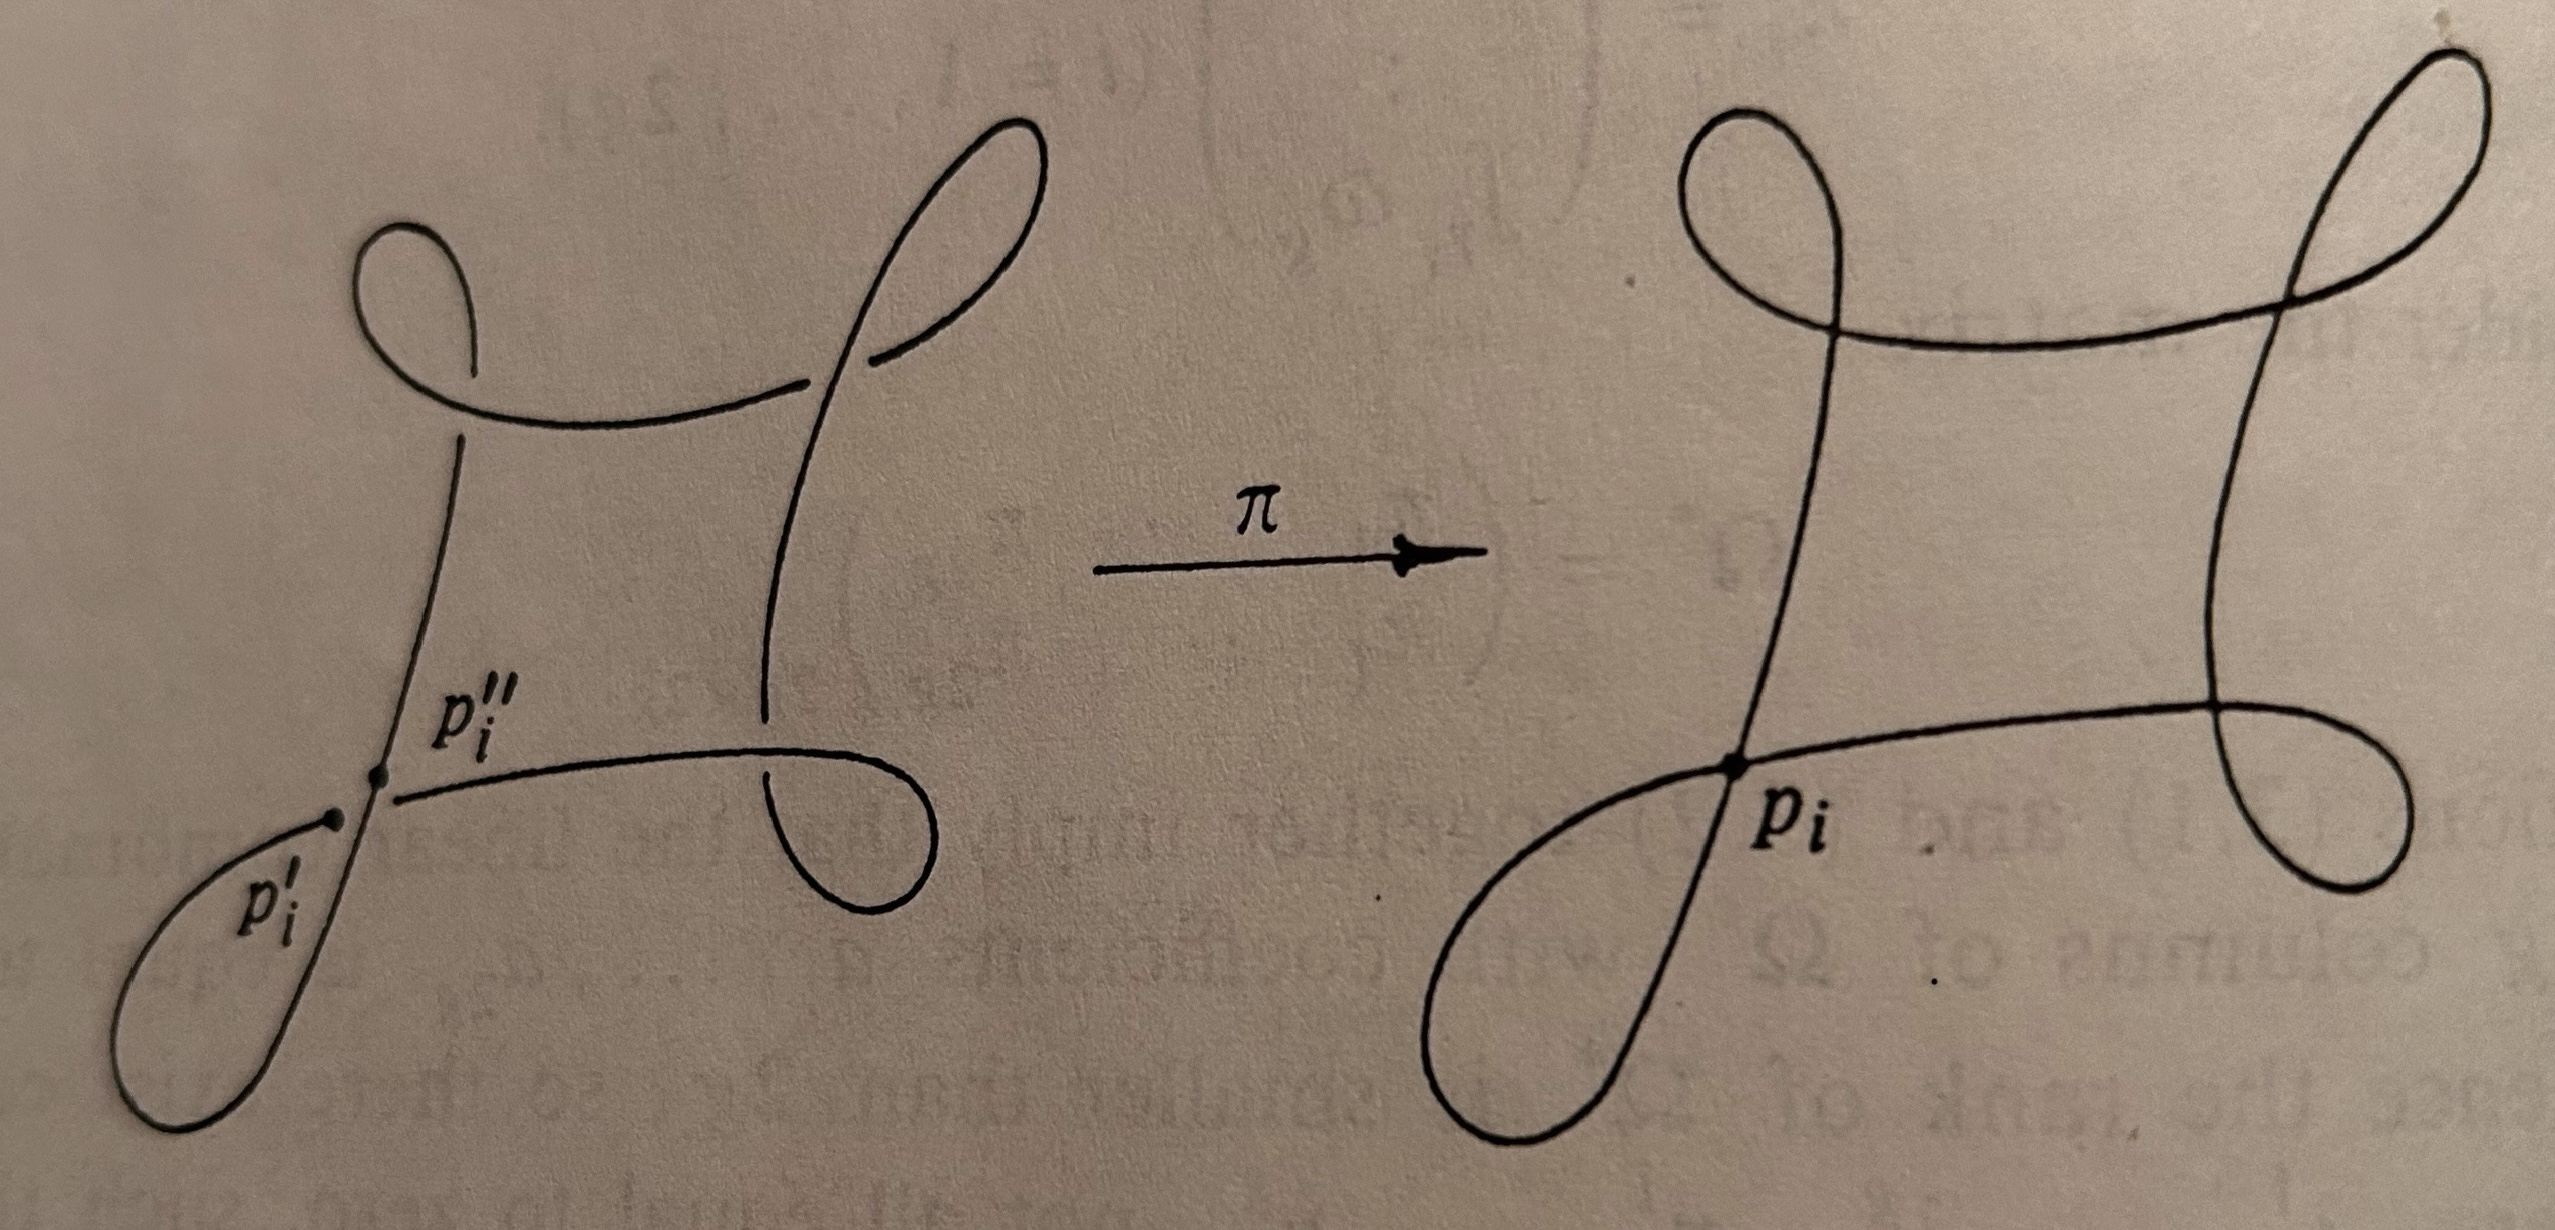
\includegraphics[width=0.8\textwidth]{images/Normalization_by_Griffiths.png}
  \caption{normalizatoin}
  \label{fig:normalization_by_griffiths}
\end{figure}
  Let $\pi{-1}(p_i) = p_i' + p_i''$. Then let:
  \[
    \Delta = \sum_{i=1}^\delta (p_i' + p_i'') \in \Div(C)
  \]
  Then by a change of coordinates in $\CP^2$, without loss of generality we may assume neither $\pi(D)$ nor
  $\pi(\Delta)$ contain the point at infinity (like in the above figure). Now, let $C'$ be given by the
  equation $F(\xi^0, \xi^1, \xi^2) = 0$, $\deg F = m$. Let $D = D'-D''$ where $D', D'' \ge 0$ and let
  \[
    \deg D' = d' \qquad \deg D'' = d''
  \]
  Let $S^n$ be the vector-space of complex homogeneous polynomials in three variables of degree $n$. Then:
  \[
    \dim S^n = \frac{1}{2} (n+1)(n+2)
  \]
  Now let's consider a polynomial $G(\xi^0, \xi^1, \xi^2) \in S^n$ satisfying:
  \begin{enumerate}
    \item $F\nmid G$
    \item $G\cdot C \ge D' + \Delta$ where $G\cdot C = (\pi^*(G(\xi^0, \xi^1, \xi^2)))$ (that is, the divisor
      induced by the zeros of $\pi^*(G)$ on $C$). Note that $G\cdot C \in \Div(C)$.
  \end{enumerate}
  We shall elaborate why we would want such a polynomial, then show such a polynomial exists. First, for $p
  \in C$, let $p' = \pi(p) \in C'$. Then a neighbourhood of $p$ gets mapped under $\pi$ into a curve component
  of $C'$ near $p'$; denote it by $B_p$. Then after a possible coordinate change, we may take $p'$ to be
  $[1:0:0]$. Label the equation after this coordinate change $G_p$. As the multiple points of $C'$ are ordinary
  double points, the equation of $B_p$ near $p'$ is:
  \[
    y = a_0 + a_1x^2  +\cdots
  \]
  Putting this into $G_p(1,x,y)$, we get a power series in terms of $x$. Now, let $n(p)$ denote the degree of
  the lowest term. We then get:
  \[
    G\cdot C = \sum_{p \in C} n(p)p
  \]
  the right hand side is certainly a finite sum. (I'll finish rest later)

\end{Proof}

\begin{cor}{Comparing Degree and Genus}{comparingDegAndGenus}
  If $d \ge g$, then
  \[
    l(D) \ne 0
  \]
  Hence if $l(D) = 0$, then:
  \[
    d \le g-1
  \]
\end{cor}

\begin{Proof}
  immediate
\end{Proof}

\begin{prop}{Meromorphic Differentials and Riemann Inequality}{meromorphicDifferentialsandRiemannInequality}
  \[
    i(D) \ge g-d-1
  \]
\end{prop}

\begin{Proof}
  Let $F,m,D', D'', d', d''$, and $\Delta$ be as in~\cref{th:riemannInequality}. \textcolor{red}{finish here}.
\end{Proof}

\begin{cor}{Comparing Degree and Genus -- Meromorphic Differential}{compDegAndGenusMeromorphicDiff}
  If $d \le g-2$, then $i(D) \ne 0$, hence if $i(D) = 0$ then
  \[
    d \ge g-1
  \]
\end{cor}

\begin{Proof}
  immediate
\end{Proof}

Finally this leads us to:

\begin{thm}{Riemann-Roch Theorem}{riemann-rochthm}
  Let $C$ be a compact Riemann surface of genus $g$ and :
  \[
    D = \sum_{i=1}^k n_ip_i \in \Div(C)
  \]
  Then:
  \[
    l(D) = d-g+i(D) +1
  \]
\end{thm}

\begin{Proof}
  see~\cite[p.118]{a.griffithsIntroductionAlgebraicCurves}

  \qn
  Let us first assume $D\ge 0$ and prove
  \[
    l(D) \le d-g+i(D) + 1
  \]
  And then take cases and judiciously use the Riemann inequality and its corollary to get the results. Suppose
  $\eta = (\eta_1, ..., \eta_k)$ where:
  \[
    \eta_i = \frac{a^{in_i}}{z_i^{ni}} + \cdots + \frac{a_{i1}}{z_i}
  \]
  is a Laurent principal part near $p_i$. The linear space consisting of all these $\eta$ is isomorphic to
  $\C^d$. Then thinking of $\eta$ as a vector in $\C^d$, consider:
  \begin{gather*}
    \Res: \C^d \times \Omega^1(C) \to \C\\
    (\eta, \omega) \mapsto \sum_{i=1}^k \Res_{p_i}(\eta_i\omega)
  \end{gather*}
  This is certainly a bilinear mapping. Let us show that:
  \[
    \Res(\eta, \omega) = 0,\ \forall \eta \in \C^d \qquad \text{if and only if} \qquad \omega \in \Omega^1(D)
  \]
  If $\omega \in \Omega^1(D)$, then $\eta_i\omega$ does not have $p_i$ as a pole for all $i = 1,..., k$,
  hence:
  \[
    \Res_{p_i}(\eta_i\omega) = 0
  \]
  and so the sum of residues is zero, giving the $\Lw$ direction. For the $\Rw$ direction, assume otherwise so
  that $\omega \in \Omega^1(C)$ such that $\Res(\eta, \omega) = 0$ for all $\eta \in \C^d$ but $\omega \notin
  \Omega^1(D)$. Then near $p_i$, let
  \[
    \omega = b_{i0}z_i^{m_i} + b_{i1}z_1^{m_i+1} + \cdots
  \]
  where $m_i \in \Z$, $b_{i0} \ne 0$. By assumption, $m_i < n_i$. Then there is a Laurent Principal part near
  $p_i$
  \[
    \xi_i = (\xi_{i1}, ..., \xi_{ik})
  \]
  such that
  \[
    \xi_{ii} = \frac{1}{z_i^{m_i+1}} \qquad \xi_{ij} = 0\ (i\ne j)
  \]
  As $m_i+1 \le n_i$, $\C^d$, by treating these as $\C^d$ we have $\xi_i \in \C^d$. However:
  \[
    0 = \Res(\xi_i, \omega) = \Res_{p_i} \frac{b_{i0}}{z_i} = b_{i0} \ne 0
  \]
  a contradiction. Thus, $m_i \ge n_i$, and so $\omega \in \Omega^1(D)$.

  Next, recall the following fact (or see exercise ref:HERE). Let $B: V\times W \to \C$ be a bilinear map
  between two finite dimensional vector spaces, in particular $\dim V = n$ and $\dim W = m$. Then $B$ is called non-degenerated if given $w \in W$, $B(v,w)
  = 0$ for all $v \in V$ implies $w = 0$. Then given $L \sse V$ satisfies $B(L\times W ) = 0$, then:
  \[
    \dim L \le n-m
  \]
  Then by the property we just found earlier about the residue map, we have a non-nondegenerate bilinear map:
  \[
    \Res_1: \C^d \times \frac{\Omega^1(C)}{\Omega^1(D)} \to \C
  \]
  Now recall we can interpret $\CL(D)/\C$ as a subspace of $\C^d$, and by what we've just shown:
  \[
    \Res_1 \left(\frac{\CL(D)}{\C}\times \frac{\Omega^1(C)}{\Omega^1(D)}\right) = 0
  \]
  Then:
  \[
    \dim \left( \frac{\CL(D)}{\C}\right) \le \dim \C^d - \dim \left(\frac{\Omega^1(C)}{\Omega^1(D)}\right)
  \]
  That is:
  \[
    l(D) -1 \le d - \dim \Omega^1(C) + i(D)
  \]
  By~\cref{th:dimOfDiffForms}, $\dim \Omega^1(C) = g$, and so we get:
  \[
    l(D)\le d-g+i(D) + 1
  \]
  This was the hardest part of the proof. We now cases cases on $l(D)$ and $i(D)$ to finish:
  \begin{enumerate}
    \item Consider $l(D) \ne 0$, $i(D) = 0$. As $l(D) \ne 0$, there exists an $f \in K(C)$ such that $(f)
      + D \ge 0$. Let $E = (f) + D$. Then $(f) = E-D$, so $E\sim D$. Then
      \[
        l(D) = l(E) \qquad i(D) = i(E) \qquad \deg D = \deg E
      \]
      Thus, we may assume  $D \ge 0$. Thus we get our inequality, and by the Riemann inequality:
      \[
        d-g+i(D) +1 = d-g+1 \overset{\text{R.}}{\le} l(D) \le d-g+1
      \]
      giving equality
    \item  Consider $l(D) \ne 0$, $i(D) \ne 0$. As $l(D) \ne 0$, we may do the same trick to assume $D\ge 0$.
      Since $i(D) \ne 0$, there exits a $\omega \in \Omega^1(C)$ such that
      \[
        (\omega) \ge D
      \]
      Let $E = (\omega) - D$ so that $E \ge 0$. Then by~\cref{pr:brill-noetherReciprocity}
      and~\cref{pr:meromorphicDifferentialsandRiemannInequality} we get:
      \[
        i(D) = l(E) \le \deg E -g+1+i(E)
      \]
      By the Poincar\'e-Hopf formula, $\deg(\omega) = 2g - 2$ so
      \[
        \deg E = \deg(\omega) - \deg(D) = 2g-2-d
      \]
      As $i(E) = l(D)$, we get:
      \[
        i(D) \le 2g-2-d-g+1+l(D)
      \]
      re-arranging and combining we  get:
      \[
        l(D) \ge d-g+i(D) + 1
      \]
      giving us the other wise
     \item Consider $l(D) = 0 $, $i(D) \ne 0$. Since $i(D) \ne 0$, there exists a $\omega \in \Omega^1(C)$ such
       that $(\omega) = D+E$ where $E \ge 0$. Then by~\cref{pr:brill-noetherReciprocity}
       \[
        l(E) = i(D) \ne 0 \qquad i(E) = l(D) = 0
       \]
       Thus, by case (1) applied to $E$ we get:
       \[
        l(E) = \deg E - g + i(E) + 1
       \]
       Note that
       \[
        \deg E = \deg(\omega) - \deg D = 2g-2-d
       \]
       Then substituting and rewriting $l(E)$, $i(E)$ as $i(D)$ and $l(D)$, we get the equality.
     \item Consider $l(D) = 0$, $i(D) = 0$. Then by~\cref{co:comparingDegAndGenus}
       and~\cref{co:compDegAndGenusMeromorphicDiff}
       \[
        d = g-1
       \]
       which is the desired equation.
  \end{enumerate}
\end{Proof}

(then do the exercises for $C = \P^1$ direct prove, and the elliptic curve exercise)

\section{Application of Riemann-Roch Theorem}\label{sec:applicationRiemannRoch}

It shall cover genus $0,1,2,3,4$.

\subsection{Genus 0}

\begin{prop}{Genus 0 then Rational}{genus0thenRational}
  Let $C$ be a compact Riemann surface of genus $0$. Then
  \[
    C \cong \P^1
  \]
\end{prop}

\begin{Proof}
  Let $p \in C$, $D = (p) \in \Div(C)$. Then:
  \[
    0 \le i(D) \le i(0) = \dim \Omega^1(C) = 0
  \]
  Thus $i(D) = 0$. By the Riemann-Roch theorem:
  \[
    l(D) = d-g+i(D) + 1 = 1-0+0+1 = 2
  \]
  Thus, $\CL(p)$ contains two linearly independent function, one of which can be chosen to be $f_1 = 1$. The
  other function must be a meromorphic function (as $C$ is a compact Riemann surface) and must have $p$ as
  a pole of order $1$; call this function $f_2$. Then by definition $f_2^{-1}(\infty) = p$. Hence it follows
  that this is a holomorphic mapping:
  \[
    f_2: C \to \P^1
  \]
  where $\deg f_2 = \#\{f_2^{-1}(\infty)\} = 1$ implying that $f_2$ is in fact biholomorphic
  (recall~\cref{lm:densInjThenBiholo}). Thus:
  \[
    C \cong \P^1
  \]
  as we sought to show.
\end{Proof}


\subsection{Genus 1}

\begin{prop}{Genus 1 Weierstrass Equation Representation}{genus1WeierstassEqn}
   Let $C$ be a compact Riemann surface of genus $1$. Then $C$ can be represented by a smooth algebraic curve
   of degree $3$ in $\P^3$
\end{prop}

\begin{Proof}
  We shall construct a holomorphic injective map $f: C \hookrightarrow \P^2$ where $f$ shall be a smooth
  algebraic curve of degree $3$. First, for any nonzero $\omega \in \Omega^1(C)$, by Poincar\'e-Hopf formula
  we have:
  \[
    \deg(\omega) = 2g - 2 = 2-2= 0
  \]
  Hence, if $\omega(p) = 0$, then it would have to have a pole, but it is holomorphic! Thus, for any $D > 0$,
  $i(D) = 0$. Thus, letting $D = 2p$, we get:
  \[
    i(D) = 0
  \]
  Thus by the Riemann-Roch theorem we have that:
  \[
    l(2p) = d-g+i(2p) + 1 = 2-1+0+1 = 2
  \]
  Hence $\CL(D)$ has non-constant meromorphic functions which only have $p$ as a singular point of order $\le
  2$. In fact, it \emph{must} be of order $2$, as by the Riemann-Roch theorem:
  \[
    l(p) = 1-1+1=  1
  \]
  Hence $\CL(p)$ only has constant functions; and so the order of any meromorphic function with single pole $p$
  is at least $2$. Let $x \in \CL(2p)$ be such a function. Then near $p$ we have:
  \[
    x = \frac{c_2}{t^2} + \frac{c1}{t} + h_1(t)
  \]
  for a local coordinate near $p$ where $t(p) = 0$ and $c_2 \ne 0$. Let's start by showing that it must be
  that $c_1 = 0$. As $\dim \Omega^1(C) = g = 1$, take a $\omega \in \Omega^1(C)$ that is nonzero so that under
  $t$
  \[
    \omega = g(t)dt \qquad g(0) \ne 0
  \]
  Then $x\omega$ has no poles other than $p$, so by the Residue Theorem (the sum of all residues is $0$):
  \[
    0 = \Res_p(x\omega) = c_1
  \]
  Thus, with a suitable change of coordinates we get:
  \[
    x = \frac{1}{z^2} + h(z)
  \]
  Note that this $x$ has many similar properties to the Weierstrass function, as we shall see later.

  Now, for any $\omega \in \Omega^1(C)$, let
  \[
    y = \frac{dx}{\omega}
  \]
  which is well defined as $\omega(p) \ne 0$ for all $p \in C$. Define:
  \begin{gather*}
    f: C \to \P^2 \\
    q \mapsto [1: x(q): y(q)] \qquad (p \mapsto [0:0:1])
  \end{gather*}
  Note that our chosen point $p$ was mapped to the point at infinity. Certainly $f$ is holomorphic, we must just show it is injective and that $f(C)$ is a curve of degree $3$.

  Starting by showing $f(C)$ is a degree $3$ curve in $\P^2$, consider $x: C \to \P^1$. Then by construction
  $x^{-1}(\infty) = 2p$. Thus:
  \[
    \deg x = 2
  \]
  Thus, the ramification can never exceed $1$, and hence the ramification index at its ramification points
  never exceeds $1$. In particular, the coefficients of every point for the ramification divisor of $x$ must
  be $1$. By the Riemann-Hurwitz formula;
  \[
    \deg R = 2(\deg x + g-1) = 2(2+1-1) = 4
  \]
  As $p$ ramified, there are $3$ other Ramification points:
  \[
    R = p_1 + p_2 + P_3 + p
  \]
  each $p_i$ being mutually distinct:

  \begin{center}
    FIG HERE
  \end{center}
  let $x(p_i) = a_i$. Let us figure out what type of ramification we have. To be succinct with tracking roots
  and poles, for a meromorphic differential form $\alpha \in K^1(C)$, let $(\alpha)_0$ and
  $(\alpha)_\infty$ represented the zeros and poles (including multiplicity) respectively. As $\omega$ has no
  zeros or poles then since $y = dx/\omega$ we get:
  \[
    (y)_0 = (dx)_0 \qquad (y)_\infty = (x)_\infty
  \]
  Hence, $(y)_0$ and $(y)_\infty$ can only contain the points of $x$ with ramification index $1$, that is
  $p_1, p_2, P_3, p$. Thus, each of these ``zero'' and ``pole'' divisors are shared between the two.

  To calculate, suppose $z_i (i = 1,2,3)$ are local coordinates near $p_i$ where $z_i(p_i) = 0$. Since the multiplicity of
  $x$ at $p_i$ is $2$,
  \[
    x - a_i = z_i^2h_i(z_i)
  \]
  where $h_i$ is a holomorphic function and $h_i(0) \ne 0$. Thus:
  \begin{align*}
   dx &= 2z_ih_i(z_i)dz_i + z_i^2 h_i'(z_i)dz_i\\
   z_i(2h_i(z_i) + z_ih_i'(z_i))dz_i
  \end{align*}
  But then evaluating at $z_i = 0$:
  \[
    (2h_i(z_i) + z_ih_i'(z_i))|_{z_i=0} = 2h_i(0) \ne 0
  \]
  and so $p_i$ is a simple zero of $dx$. For the pont $p$, choosing a local coordinate function $z$ near $p$
  as we did before we get:
  \[
    x = \frac{1}{z^2} + h(z)
  \]
  Neurally, $dx$ has $p$ as a pole of order $3$, and so we found:
  \[
    (y)_0 = p_1 = P_2 + P_3 \qquad (y)_\infty = 3p \qquad (y) = p_1 + p_2 + p_3 - 3p
  \]
  We now know the roots/pole information our desired function must have. Let $g(x) \in K(\P^1)$ be given by:
  \[
    g(x) = (x-a_1)(x-a_2)(x-a_3)
  \]
  Considering $g$ as a function on $C$ (that is $x^*g$), then as near the points $p_i$ and $p$ in coordinates
  $z_i$ and $z$:
  \[
    x-a_i = z_i^2h_i(z_i) \qquad x = \frac{1}{z^2}h(z)
  \]
  we get:
  \[
    (g)_0 = 2p_1 + 2p_2 + 2p_3 \qquad (g)_\infty = 6p
  \]
  since each $p_i$ takes $p_i$ as a zero of order $2$, an near $p$ every $(x-a_i)$ takes $p$ as  pole of order
  $2$.

  Now, we see that the divisor of $g$ is just the divisor of $y^2$, and so:
  \[
    \left(\frac{y^2}{g}\right) = 0
  \]
  showing $y^2/g$ is holomorphic on $C$, and as $C$ is compact $y^2/g = a\in \C$ where $a\ne 0$. To choose
  a better constant replace $y$ by $y/\sqrt{a}$. Then we get:
  \[
    y^2 = g(x)
  \]
  But now, we just showed that under $f$ that $C$ lies in the image of a curve of degree $3$:
  \[
    C' = \set{[1:x:y] \in \P^2}{y^2-g(x) = 0} \cup \{[0:0:1]\}
  \]
  Giving us the degree. Let us now check that $f$ is an injective mapping except at $\infty$.

  To that end, we shall need a bit more structure on $C$. We shall define a natural involution map on $C$. Let
  \begin{gather*}
    j: C \to C\\
    q_1 \mapsto q_2
  \end{gather*}
  where $q_1, q_2 = x^{-1}(p_r)$ are an arbitrary $p_r \in C'$ (where I chose subscript $r$ for no particular
  reason, we're running out of letters).  Then certainly $j^2 = \id$. It is thus it's own inverse, and so it
  is easy to verify it is an automorphism. Using this, we shall show some properties of $j^*$ on $K(C)$,
  $K^1(C)$ and  $\Omega^1(C)$. Certainly by definition of $j$:
  \[
    j^*(x) = x \qquad j^*(d ) =dx
  \]
  Let's show $j^*y = -y$. As $y = dx/\omega$:\[
    j^*y = \frac{j^*(dx)}{j^*(\omega)}= \frac{dx}{d^*(\omega)}
  \]
  Hence, we show $j^*(\omega) = -\omega$. As $\dim \Omega^1(C) = g= 1$, we get $\Omega^1(C) \cong \C$. Then
  notice that $j$ can be thought of as a linear transformation on $]C$ so that $j^2 = 1$  implies $(j^*)^2 =
  1$, (hence it is diagonalizable) hence the eigenvalues of $j^*$ are either $1$ or $-1$. Suppose $j^*$ has
  eigenvalue $1$ so that $j^*\omega =\omega$. Then there exists a holomorphic differential $\phi$ on $\P^1$ such that
  \[
    \omega = \phi\circ x = x^*\phi
  \]
  (exercise). But there is no nonzero holomorphic differential on $\P^1$, hence $j^*\omega = -\omega$.

  With the properties of $j$ established, consider $q_1, q_2 \in C$ where $f(q_1) = f(q_2)$. We want to show
  that $q_1 = q_2$. Naturally if either $q_1, q_2$ is $p$ then by construction $f(q_1) = f(q_2) = \infty$ and
  so $q_1 = q_2 = p$; thus we assume neither $q_1, q_2$ is $p$. By definition:
  \begin{align*}
    f(q_1) &= [1:x(q_1): y(q_1)]\\
    f(q_2) &= [2:x(q_2): y(q_2)]\\
  \end{align*}
  and as these are equal $x(q_1) = x(q_2)$ and $y(q_1) = y(q_2)$. Now if $q_1 \ne q_2$, as $x(q_1) = x(q_2)$
  it must be that $j(q_1) = q_2$. Thus, we have by definition of the pullback:
  \[
    j^*y(q_1) = y(q_2)
  \]
  however as $j^*(y) = -y$
  \[
    j^*y(q_1) = -y(q_1) = -y(q_2)
  \]
  and so
  \[
    y(q_2) = -y(q_2)
  \]
telling us $y(q_2) = 0$. But $(y)_0 = p_1+p_2+p_3$, so $q_2 \in \{p_1, p_2, p_3\}$. Thus:
\[
  q_1 = j(q_2) = q_2
\]
but this contradicts $q_1 \ne q2$, thus it must be that they are equal, showing $f$ is injective.

Let's now show surjectivity. We shall use a connectedness argument. First, $y^2-g(x) = 0$ is certainly an
irreducible polynomial, hence it forms an irreducible subset, hence a connected subset. Next, $C$ is compact,
and as $f$ is holomorphic $f(C)$ is closed. As $f$ is holomorphic, $f(C)$ is also open (by the holomorphic
open mapping theorem), and so $f(C) = C'$.

Finally, we prove $C'$ is smooth. We can show this directly by computing . By everything shown so far, we know
that the projective equation of $C'$ can be written as:
\[
  F = \xi^0(\xi^2)^2 - (\xi^1 - a_1\xi^0)(\xi^1-a_2\xi^0)(\xi^1-a_3\xi^0) = 0
\]
Thus:
\begin{align*}
\frac{\partial F}{\partial \xi^0} &= (\xi^2)^2 + a_1(\xi^1 - a_2\xi^0)(\xi^1 - a_3\xi^0)\\
                                  &+ a_2(\xi^1 - a_1\xi^0)(\xi^1 - a_3\xi^0)\\
                                  &+ a_3(\xi^1 - a_1\xi^0)(\xi^1 - a_2\xi^0)
\end{align*}
\begin{align*}
  \frac{\partial F}{\partial \xi^1} &= -(\xi^1 - a_2\xi^0)(\xi^1 - a_3\xi^0)\\
                                    &-(\xi^1 - a_1\xi^0)(\xi^1 - a_3\xi^0)\\
                                    &-(\xi^1 - a_1\xi^0)(\xi^1 - a_2\xi^0)
\end{align*}
\[
  \frac{\partial F}{\partial \xi^2} = 2\xi^0\xi^2
\]

If $\partial F/\partial \xi^i$ $(i = 1, 2, 3)$ are all zero, by the Euler formula, $F = 0$. Now from
\[
2\xi^0\xi^2 = 0
\]
we get
\[
\xi^0(\xi^2)^2 = 0,
\]
and substituting this expression into $F = 0$, we also get
\[
(\xi^1 - a_1\xi^0)(\xi^1 - a_2\xi^0)(\xi^1 - a_3\xi^0) = 0.
\]

At least one of the three factors on the left side of this expression is therefore equal to 0. Having only one factor equal to 0 however, contradicts
\[
\frac{\partial F}{\partial \xi^1} = 0.
\]

Thus at least two of the factors are equal to 0. But then $\xi^0 = \xi^1 = 0$ because $a_1, a_2, a_3$ are mutually distinct. Substituting into
\[
\frac{\partial F}{\partial \xi^0} = 0,
\]
we get $\xi^2 = 0$, i.e., we get
\[
\xi^0 = \xi^1 = \xi^2 = 0,
\]
and this is impossible. Thus, $C'$ is smooth. As $f$ is biholomorphic, we have that $C$ is biholomorphic to
a smooth degree $3$ curve, as we sought to show.
\end{Proof}

\subsection{Genus $\ge 2$: Canonical Map}

In higher dimensions, there are generally many kinds of mapping from a compact Riemann surface into an
$n$-dimensional projective space. However all compact Riemann surface of genus $g \ge 2$, they exits as
special holomorphic mapping from this compact Riemann surface into $\P^{g-1}$ that is called he
\emph{canonical map}.


\index{Canonical Map}
\begin{defn}{Canonical Map}{cannonicalMap}
  Let $C$ be a compact Riemann surface of genus $g\ge 2$ an $\{\omega_1, ..., \omega_g\}$ a basis for
  $\Omega^1(C)$. Then:
  \begin{align*}
    \phi_K: C \to \P^{g-1}\\
    p \mapsto [\omega_1(p): \cdots : \omega_g(p)]
  \end{align*}
\end{defn}

Note that this is well-defined. It is certainly not coordinate dependent, and if, for the sake of
contradiction, there is a $p$ where $\omega_i(p) = 0$ for all $p$ (which implies $p$ maps to $[0:\cdots: 0]$
which doesn't exist), then notice that $\Omega^1(p) = \Omega^1(C)$ so
\[
  i(p) = \dim \Omega^1(C) = g
\]
and by the Riemann Roch-theorem
\[
  l(p) = 1-g+g+1=  2
\]
and so there exits nonconstant meromorphic function $f \in \CL(p)$ where $f^{-1}(\infty) = p$. Thus
\[
  \deg f  = 1
\]
giving us that $f:  \to \P^1$ is an isomorphism, but that is not possible as $\P^1$ has genus $0$.

\begin{prop}{Non-degeneracy of Canonical Map}{non-degeneracyofCannonicalMap}
  Let $\phi_K$ be the canonical map. Then $\phi_K$ is non-degenerate.
\end{prop}

\begin{Proof}
  Assume $\phi_K$ is degenerate so that there exists $\lambda_\alpha \in \C$ not all zero st for all $p \in C$
  \[
    \sum_\alpha^g \lambda_\alpha\omega_\alpha(p) = 0
  \]
  Then:
  \[
    \sum_\alpha^g \lambda_\alpha\omega_\alpha
  \]
  contradicting that $\{\omega_1, ..., \omega_g\}$ is a basis of $\Omega^1(C)$, as we sought to show.
\end{Proof}

\begin{prop}{Degree 2 Mapping Condition}{deg2MappingCond}
  Let $C$ be a Riemann surface of genus $g\ge 2$ and let $\phi_K$ be the canonical mapping. Then if
  \[
    \phi_K(p) = \phi_K(q)
  \]
  for some distinct $p,q \in C$, then there exists a holomorphic mapping of degree $2$ from $C$ into $\P^1$
\end{prop}

\begin{Proof}
  If $\phi_K(p)  = \phi_K(q)$ ,then $\omega_\alpha(p) = \lambda\omega_\alpha(q)$ for all $\alpha = 1,..., g$
  for some $0 \ne \lambda  \in \C$. Let $D = p+q$. Let us find $i(D)$. We shall start by showing that:
  \[
    \Omega^1(D)  = \Omega^1(p)
  \]
  Indeed, for any $\omega \in \Omega^1(C)$, if
  \[
    \omega = \sum_{\alpha=1}^g \mu_\alpha\omega_\alpha
  \]
  for $\mu_\alpha \in \C$, $\alpha = 1,..., g$, then:
  \begin{align*}
    \omega(p) = 0 &\LRw \sum_{\alpha=1}^g \mu_\alpha\omega_\alpha(p) = 0\\
      &\LRw \sum_{\alpha=1}^g \lambda\mu_\alpha\omega_\alpha(q) = 0\\
      &\LRw \omega(q) = 0
  \end{align*}
  Thus, $\Omega^1(p) = \Omega^1(p+q) = \Omega^1(D)$. Hence, to calculate $i(D)$ it suffices to calculate
  $i(p)$.

  To that end, consider :
  \[
    \lambda_2\omega_1(p) + \lambda_2\omega_2(p) + \cdots + \lambda_g\omega_g(p) = 0
  \]
  for $\lambda_1, ..., \lambda_g \in \C$. Note not all these could be zero or else we would have a point
  map to $[0:\cdots :0]$. Hence, this linear equation \emph{must} have $g-1$ linearly independent
  solution vectors $(\lambda_1, ..., \lambda_g) \in \C^g$, giving rise to $g-1$ linearly independent
  elements in $\Omega^1(p)$. Thus:
  \[
    i(D) = i(p) = g-1
  \]
  Applying the Riemann-Roch there to $D = p+q$, we get:
  \[
    l(D) = 2-g+(g-1)+1 = 2
  \]
  Thus, there exist a  nonconstant meromorphic function $f \in \CL(p+q)$. Thus there is a holomorphic $f: C
  \to \P^1$where $f^{-1}(\infty) = p+q$. Note that $f^{-1}(\infty)$ cannot e a single point $p$ or
  $q$ otherwise we get $C \cong \P^1$, contradicting the fact that the genus $g$ of $C$ is $\ge 2$. Thus,
  it must be that:
  \[
    \deg f = 2
  \]
  as we sought to show.
\end{Proof}

This gives a rough division of Riemann surface of genus $g> 1$:

\index{Hyperelliptic and Nonhyperelliptic}
\begin{defn}{Hyperelliptic and Nonhyperelliptic}{hyperellipticandNonhyperelliptic}
  Let $C$ be a compact Riemann surface of genus $g \ge 2$. Then it is \emph{hyperelliptic}if there
  exists a holomorphic mapping of degree $2$ $f: C \to \P^1$. Otherwise, $C$ is said to be
  \emph{nonhyperelliptic}.
\end{defn}

We can deal with the nonhyperelliptic example holistically and then see the hyperelliptic examples by
examining different genera:

\index{Canonical Curve}
\begin{defn}{Canonical Curve}{cannonicalCurve}
  Let $C$ be a nonhyperelliptic compact Riemann surface of genus $g \ge 2$ with canonical map $\phi_K:
  C \to \P^{g-1}$. Then
  \[
    \phi_K(C) \sse \P^{g-1}
  \]
  is called the \emph{canonical curve}.
\end{defn}
Note that we put $g\ge 2$, but we shall show shortly that all $g= 2$ compact Riemann surface are
hyperelliptic, but this shall not necessarily be the case for $g\ge 3$.

\begin{prop}{Canonical Curve Smooth}{cannonicalCurveSmooth}
  Let $C$ be a nonhyperelliptic compact Riemann surface. Then the canonical map $\phi_K$ is injective and
  $\phi_K(C)$ is smooth.
\end{prop}

\begin{Proof}
  \Cref{pr:deg2MappingCond} show's $\phi_K$ must be injective, it remains to show $\phi_K$ is
  smooth.

  \cite[p.136]{a.griffithsIntroductionAlgebraicCurves}
\end{Proof}


\subsection{Hyperelliptic Compact Riemann Surfaces}\label{sec:hyperellipticCompactRiemannSurface}

\begin{prop}{Algebraic Characterization of Hyperelliptic Riemann Surface}{charHyperellitpicRiemannSurface}
  Let $C$ be a hyperelliptic compact Riemann surface. Then it can be represented as the normalization of
  a plane algebraic curve of degree $2g+2$ where $g$ is the genus of $C$. By a suitable linear projection,
  this plane curve will be a $2$-sheered covering of a straight line (i.e. $\C$).
\end{prop}

\begin{Proof}
  Let $C$ be a hyperelliptic compact Riemann surface of genus $g$. We shall construct a holomorphic mapping $f:
  C \to \P^2$ such that $f(C)$ can be given by a plane algebraic curve of degree $2g+2$.

  As $C$ is hyperelliptic, the exist a degree $2$ holomorphic mapping $x: C \to \P^1$. Let $R$ be the
  ramification divisor of $x$. By the Riemann-Hurwitz formula (\cref{th:riemann-hurwitzFormula}):
  \[
    \deg R = 2(2+g-1) = 2g+2
  \]
  As $x$ is degree $2$, the coefficients of every point in $R$ must be equal to $1$, hence we must have:
  \[
    R = p_1 + p_2 + \cdots + p_{2g+2}
  \]
  where each $p_i$ is distinct on $C$. Now suppose:
  \[
  x^{-1}(\infty) = p+q \qquad x(p_i) = a_i
  \]
  so that $x$ can be visualized as:
  \begin{center}
    FIG HERE
  \end{center}
  Then as in~\cref{pr:genus1WeierstassEqn} we can define $j: C \to C$ $j(q_1) = q_2$. Just like before, $j \in
  \Aut(C)$ and $j^2 = 1$. Define again $j^*: K(C) \to K(C)$ by $j^*(a) = a\circ j$, which like before can be
  extended to $K^1(C)$ and restricted down to $\Omega^1(C)$. Then as $\Omega^1(C) \cong \C^g$, this is
  a linear involution of $C^g$ with eigenvalues $1$ or $-1$. If the eigenvalue is $1$, then the eigenvector
  corresponding to $1$ will be a holomorphic differential form, inducing a nontrivial differential form on
  $\P^1$ a contradiction. Thus it must be that :
  \[
    j^*: \Omega^1(C) \to \Omega^1(C) \qquad \omega \mapsto -\omega
  \]

  With the setup complete, let us show that such a function does exist by the Riemann-Roch Theorem. Let
  \[
    D = (g+1)p + (g+1)q \in \Div(C)
  \]
  Recall that for nay $\omega \in K^1(C)$ by the Poincar\'e-Hopf formula $\deg(\omega) = 2g-2 < \deg G$, and
  so it cannot be that $(\omega) - D \ge 0$, and so $i(D) = 0$. Then by Riemann-Roch:
  \[
    l(D) = (2g+2)-g+1 = g+3
  \]
  Thus
  \[
    \CL(D) \cong \C^{g+3}
  \]
  As $x(p) = x(q) = \infty$, it must be that $j(D) = D$, so $j^*$ can be seen as a linear transformation on
  $\CL(D)$. Then a $(j^*)^2 = 1$ and $j^*$ also has eigenvalues $\pm 1$, we can split $\CL(D)$ into
  eigenspaces:
  \[
      \CL(D) = \CL(D)^+ \oplus \CL(D)^-
  \]
  where $\CL(D)^+$ and $\CL(D)^-$ are the eigenspace for eigenvalue $+1$ and $-1$ respectively. Note that the
  meromorphic functions in $\CL(D)^+$ can be factored as the composition of $x$ and a meromorphic function on
  $\P^1$ with pole poles only at $p,q$, and the order of the pole at either point not exceeding $g+1$. Thus,
  as meromorphic functions on $C$, the functions $1,x,x^2, ..., x^{g+1}$ form a basis for $\CL(D)^+$. Thus:
  \[
    \dim \C(D)^+ = g+2
  \]
  As $l(D) = g+3$, it follows that
  \[
    \dim \C(D)^- = 1
  \]
  In particular, there exists a meromorphic function $y \in \CL(D)$ such that
  \[
    j^*(y) = -y
  \]
  With this build-up, let us compare divisors to prove that there exists a function $g(x) =
  (x-a_1)(x-a_2)\cdots (x-a_{2g+2})$ such that
  \[
    y^2 = cg(x)
  \]
  where $0\ne c \in \C$. Let's first find $(y^2)$, in particular it suffices to find $(y)$. since
  \[
    j^*(y) = -y \qquad j(p_i) = p_i \qquad (i = 1,2,...,2g+2)
  \]
  we get:
  \[
    y(p_i) = -y(p_i)
  \]
  and so
  \[
    y(p_i) = 0
  \]
  Thus
  \[
    \deg(y)_0 \ge \deg \left(\sum_{i=1}^{2g+2}p_i\right) = 2g+2
  \]
  But by the Residue Theorem
  \[
    \deg(y)_0 = \deg(y)\infty = 2g+2
  \]
  Thus
  \[
    (y)_0 = \sum_{i=1}^{2g+2} p_i \qquad (y)_\infty = D
  \]
  For $(g(x))$, by definition $(x)_\infty = p+q$ and $(x-a_i)_{\infty} = p+q$ for all $i = 1,2..., 2g+2$.
  Thus:
  \[
    (g(x))_\infty = (2g+2)p + (2g+2)q = 2D
  \]
  Giving the pole divisor. For the root divisor, suppose $z_i$ are local coordinate near $p_i$ for each $i$
  where $z_i(p_i) = 0$. Then:
  \[
    x-a_i = z_i^2h_i(z_i)
  \]
  where $h_i(0) \ne 0$ is holomorphic. But then:
  \[
  (g(x))_0 = \sum_{i=1}^{2g+2}2p_i
  \]
  and so $(y^2) = (g(x))$, giving that $y^2/g(x)$ is holomorphic on $C$, which as is compact makes $y^2/g(x)
  = c\ne 0$ constant. By replacing $y$ with $y/\sqrt{c}$ we get
    \[
      y^2 = g(x)
    \]
    From this, we can define the map:
    \begin{align*}
      f&: C \to \P^2\\
      t &\mapsto [1: x(t): y(t)]\\
      p,q &\mapsto [0:0:1]
    \end{align*}
    As $C$ is connected, the solution to an algebraic equation is irreducible (hence connected), $f$ is
    holomorphic (hence an open map) and $C$ is compact (hence $f$ is a closed map), it must be that $f$ is
    surjective.

    Finally, it is easy to see that each $a_I$ are distinct, hence $C$ is smooth in $\C^2 = \{[1:x:y] \in
    \P^2\}$ but singular at $[0:0:1]$ (which distinguishes from the case of $g=1$). A linear projection $(x,y)
    \to x$ gives the $2$-sheered covering, giving everything asked for by the proposition, completing the
    proof.
\end{Proof}


\begin{prop}{Canonical Map -- Hyperelliptic Case}{canonicalMap--HyperellipticCase}
  Let $C$ be a hyperelliptic curve and let $x,y$ be as in~\cref{pr:charHyperellitpicRiemannSurface}. Then
  \[
    \omega_1 = \frac{dx}{y},\ \omega_2 = \frac{(xdx)}{y},\ ...,\ \omega_g = \frac{(x^{g-1}dx)}{y}
  \]
  forms a basis for $\Omega^1(C)$.
\end{prop}

\begin{Proof}
  \cite[p.142]{a.griffithsIntroductionAlgebraicCurves}
\end{Proof}

We thus get a very simple expression for the canonical map:
\begin{gather*}
  \phi_K: C \to \P^{g+1}\\
  t \mapsto [1: x(t): \cdots : x(t)^{g-1}]
\end{gather*}

Hence, $\phi_K$ factors in the following way:
\[
\begin{tikzcd}
                                      & \P^{g-1}            \\
C \arrow[r, "x"] \arrow[ru, "\phi_k"] & \P^1 \arrow[u, "r"]
\end{tikzcd}
\]
where
\begin{gather*}
  r: \P^1 \to \P^{g-1}\\
  x \mapsto [1:x:\cdots: x^{g-1}]
\end{gather*}

Note that the converse of~\cref{pr:charHyperellitpicRiemannSurface} is true: given any $2g+2$ mutually distinct complex numbers $a_1, a_2, ...,
a_{2g+2}$, and letting:
\[
  C' = \{y^2 = \prod{i=1}^{2g+2}(x-a_i)= 0 \}\cup [0:0:1] \sse \P^2
\]
then the normalization of $C$ of $C'$ is a hyperelliptic compact Riemann surface of genus $g$, giving an
equivalence. Combining this with the commutative diagram given above, we see that $C$ is uniquely determined
by the equivalence of vectors in $\C^{2g+2}$ with (pairwise) distinct coordinates:
\[
  \{(a_1, ..., a_{2g+2})\}
\]
where $(a_1, ..., a_{2g+2})\sim (b_1, ..., b_{2g+2})$ if each coordinate is related by the same linear automorphisms
of $\P^1$, that is there exists $a,b,c,d \in \C$ $(ad-bc \ne 0$) such that
\[
  \frac{aa_i + b}{ca_i+d} = b_i \qquad (i = 1,2,..., 2g+2)
\]
(recall the classification of $\Aut(\P^1)$). Naturally, if replaced by $\lambda a,\lambda b,\lambda c,\lambda
d$ the result is unchanged, hence without loss of generality we may assume one of them is fixed.


\subsection{Genus 2 always hyperelliptic}

\begin{prop}{Genus 2 is Hyperelliptic}{genus2isHyperelliptic}
  Let $C$ be a compact Riemann surface of genus $2$. Then $C$ is hyperelliptic.
\end{prop}

\begin{Proof}
  Let $C$ be a compact Riemann surface of genus $2$. Then by~\cref{pr:deg2MappingCond} it suffices to show
  that $\phi_K$ is not injective. But if $\phi_K: C \to \P^{g-1}=\P^1$ were injective, $C$ would have genus $0$,
  completing the proof.
\end{Proof}

Thus, we always get $C$ in $\P^1$ as:
\[
  y^2 = \prod_{i=1}^6 (x-a_i)
\]
for pairwise distinct $a_1, .., a_6$ and forms
\[
  \omega_1 = \frac{dx}{y} \qquad \omega_2 = \frac{xdx}{y}
\]
where:
\[
  \phi_: C \to \P^1 \qquad t \mapsto [\omega_1: \omega_2] = [1: x(t)]
\]

\subsection{Genus 3}

We shall see in (it says at \cite[p.212]{a.griffithsIntroductionAlgebraicCurves}) that almost all genus 3
curves are canonical curves (it will be because any smooth forth-degree plane algebraic curve (where $2g-2=4$)
has genus $g= 3$ and hence is canonical). Let us start by showing that the canonical curve of genus $3$ is a smooth plane
algebraic curve of degree $3$.

let $H\sse \P^n$ be a hyperplane given by:
\[
  L(\xi) = \sum_{i=0}^n l_i\xi^i = 0
\]
Let $C$ be a smooth algebraic curve in $\P^n$. Let $H$ not contain any irreducible branches of $C$.  Then pick
the elements of $\Div(C)$ in the following way. Choose a generic linear function:
\[
  L'(\xi) = \sum_{i=0}^n l_i' \xi^i
\]
where by generic we mean:
\[
  \{L' = 0\} \cap C \cap \{L=0\} = \emptyset
\]
Then we get:
\[
  \frac{L}{L'} \in K(\P^n) \qquad \frac{L}{L'}|_C \in K(C)
\]
Then the set of all the zeros of $(L/L')|_C$ is given a name


We give a name to this set:

\index{Hyperplane Section of Riemann Surface}
\begin{defn}{Hyperplane Section of Riemann Surface}{hyperplaneSecRiemannSurface}
  Let $C,H$ be as above. Then:
  \[
    H\cdot C = \left( \left.\frac{L}{L'}\right|_C\right)_0
  \]
  is the \emph{hyperplane section} of $C$.
\end{defn}

Intuitively:
\[
  H\cdot C = C\cap \{L(\xi) = 0\}
\]
Certainly this definition is independent of choice of $L'$.
\index{Degree of Smooth Curve}
\begin{defn}{Degree of Smooth Curve}{degofSmoothCurve}
  Let $C$ be a smooth curve in $\P^n$. Then $\deg(H\cdot C)$ is called the \emph{degree} of $C$ and is denoted
  $\deg C$.
\end{defn}

This too is well-defined as it is independent of choice of hyperplane $H$ since if there exists another $H_1$:
\[
  \deg (H_1\cdot C) = \deg \left(\left.\frac{L_1}{L'}\right|_C\right)_0 = \deg
    \left(\left.\frac{L_1}{L'}\right|_C\right)_\infty = \deg \left(\left.\frac{L}{L'}\right|_C\right)_\infty
        =\deg \left(\left.\frac{L}{L'}\right|_C\right)_0  = \deg(H\cdot C)
\]
Note that when $n = 2$, then $H$ is a straight line in $\P^2$ not containing any irreducible curve components
of $C$, and so by B\'ezout's theorem we know the curve degree is just the same as the plane curve degree given
earlier.

In this section, we shall identify any nonhyperelliptic compact Riemann surface of genus $g > 1$ with its
image under the canonical map, that is the canonical curve in $\P^{g-1}$ which is a smooth surface. We can
do this as $C$ is nonhyperelliptic and hence the canonical map is injective.

\begin{prop}{Degree and Genus}{degandGenus}
  Let $C$ be a canonical curve of genus $g$. Then:
  \[
    \deg C = 2g-2
  \]
\end{prop}

\begin{Proof}
  Let $\omega_1,..., \omega_g$ be a basis for $\Omega^1(C)$ so that
  \[
    C = \set{[1w_1(p), ..., \omega_g(p)]}{p \in C}
  \]
   Suppose:
   \[
     H = \left\{ \sum_{i=0}^{g-1} l_i\xi^i=0\right\} \qquad H' = \left\{ \sum_{i=0}^{g-1} l_i'\xi^i=0\right\}
   \]
   Then by going through the definition we see that  $H\cdot C = (\omega)_0$ where $\omega = \sum_{i=0}^{g-1}
   l_i\omega_i$. As $\omega \in \Omega^1(C)$, $(\omega)_0 = (\omega)$, and hence:
   \[
    H\cdot C = (\omega)
   \]
   Thus
   \[
    \deg C  =\deg(H\cdot C) = \deg(\omega) = 2g-g
   \]
   as we sought to show.
\end{Proof}

\begin{prop}{Genus 3 By Degree 4 Curve}{genus3ByDeg4Curve}
  Let $C$ be a canonical curve of genus $3$. The n it is a smooth plane algebraic curve of degree $4$.
\end{prop}

\begin{Proof}
  It is smooth by~\cref{pr:deg2MappingCond}. As the canonical curve of genus $3$ must be in $\P^2$, by the proceeding we have:
  \[
    \deg(C) = 2g-2 = 2\cdot 3 - 2 = 4
  \]
  as we sought to show.
\end{Proof}

Note that if $F$ is a degree $4$ algebraic curve, then by the genus formula:
\[
  g = \frac{(d-1)(d-2)}{2} = \frac{3\cdot 2}{2} = 3
\]
From this we can do the same classification trick as in section~\ref{sec:hyperellipticCompactRiemannSurface}
to show that the converse is mostly true (having to take into account that some canonical embeddings are not
injective). Thus, it is as to verify that
\[
  F(x, y, z) = x^4 + y^4 + z^4 + \lambda x^2 y^2 + \mu y^2 z^2 + \nu z^2 x^2
\]
is a canonical curve.



\subsection{Genus 4}

Canonical genus $4$ curves have the amazing property that they can be characterized by the intersection of
quadric\footnote{I've not seen the word ``quadric'' before. It means a degree $2$ hypersurface embedded in
$D$ dimensions. Quadratic seems perfectly fine, but it seems that quadric is just a little more specific} and
a cubic hypersurface in $\P^3$.

Just like before, suppose $C$ Is a smooth algebraic curve in $\P^n$ and $H = \{\xi^0 = 0\}$ is a hypersurface.
Let $D = H\cdot C  \in \Div(C)$.  Notice that $\bigoplus_{k=0}^\infty \CL(kD)$ and $\C[\xi^0, ..., \xi^n]$ are
graded rings. Let $F(\xi) \in \C[\xi^0, ..., \xi^n]$ be a homogeneous polynomial and define:
\[
  r(F(\xi)) = \left.\frac{F(\xi)}{\left(\xi^0\right)^k}\right|_{C} \in \CL(k(D))
\]
Then extended $r$ linearly to all of $\C[\xi^0, ..., \xi^n]$, we get  ring homomorphism:
\[
  r: \C[\xi^0, ...,\xi^n] \twoheadrightarrow \bigoplus_{k=0}^\infty \CL(kD)
\]
I claimed this map is surjective; this was shown in~\cite{NateAlgGeo} (but a judicious application of Noether
Theorem also works).

\textcolor{red}{I'l finish typing this up later: } \cite[p.148]{a.griffithsIntroductionAlgebraicCurves}

\subsection{Abel's Theorem and its Applications}


Let $C$ be ea compact Riemann surface of genus $g\ge 1$. Then $H_1(C, \Z)$ is a free abelian group of rank
$2g$. Choose a canonical basis $\gamma_1, \gamma_2, ..., \gamma_{2g-1}, \gamma_{2g}$ for $H_1(C, \Z)$
satisfying the intersection requirements:
\[
  \gamma_i\cdot \gamma_{g+1} = 1 \qquad \gamma_{g+i}\cdot \gamma_i = -1
\]
for all $i$, and $0$ otherwise; that is it is the usual vertical and horizontal circles around the handles
when visualized in $\R^3$. Recall the period vector:
\[
  \pi_j = \begin{pmatrix}
    \int_{\gamma_j} \omega_1\\
  \vdots\\
  \int_{\gamma_j}\omega_g\\
  \end{pmatrix} \in \C^g
\]
 for $j = 1, ..., 2g$. Recall that we proved that this vector is well-defined as the paths are closed and that
 the period matrix is nonsingular (\cref{pr:periodMatrixNonsingular}). Thus, with $\Z$-coordinates, we get
 a lattice in $\C^g$:
 \[
   \Lambda = \set{\sum_{j=1}^{2g} m_j\pi_j}{m_j \in \Z} \sse \C^g
 \]
We thus can define the following:

\index{Jacobian Variety}
\begin{defn}{Jacobian Variety}{jacobianVariety}
  Let $C$ be a compact Riemann surface. Then the $g$-dimensional complex torus $\C^g/\Lambda$ is called the
  \emph{Jacobian variety} of $C$ and will be denoted $J(C)$.
\end{defn}

This variety will be useful for find ending when are divisor principal, give a measure of the lack thereof.
Namely, given a $D \in \Div(C)$, does there exist a $f \in K^*(C)$ such that
\[
  (f) = D
\]
First off, as we are working over compact Riemann surfaces, we can look at divisor of degree $0$. Let:
\begin{gather*}
  \deg: \Div(C) \to \Z\\
  D \mapsto \deg D
\end{gather*}

Let $\Div^0(C) = \ker(\deg)$. Then if $(f) = D$, it must be that $D \in \Div^0(C)$. The converse is not always
true, and Abel's theorem will outline exactly how to associate these two.

To that end, let us start by defining a map from $\Div(C)$ to $J(C)$. Let $q \in C$ be any fixed point and let $\omega
\in \Omega^1(C)$ be a holomorphic differential. Then for a point $p \in C$, we can define:
\begin{equation}\label{eq:intDiff}
  \int_q^p \omega
\end{equation}
Sine there is nontrivial winding, the difference of two paths from $q$ to $p$ is a homology class that can be
written as
\[
  \sum_{j=1}^{2g} m_j\gamma_j
\]
hence two values of equation~(\ref{eq:intDiff}) will differ by:
\[
  \sum_{j=1}^{2g} m_j \int_{\gamma_j} \omega
\]
By letting $\omega$ run through the basis of $\Omega^1(C)$, we get the following:
\index{Abel-Jacobi Map}
\begin{defn}{Abel-Jacobi Map}{abel-JacobiMap}
  Let $C$ be a compact Riemann surface, $q \in C$. Then the \emph{Abel-Jacobi map}
  \[
    u: \Div(C) \to J(C)
  \]
  is given by:
  \[
    u(D) = \begin{pmatrix}
      \sum_{i=1}^k n_i \int_q^{p_i} \omega_1\\
    \vdots\\
    \sum_{i=1}^k n_i \int_q^{p_i}\omega_g\\
    \end{pmatrix}
  \]
  where $D = \sum_{i=1}^k n_ip_i$.
\end{defn}

Certainly this is a homomorphism for if $D = \sum_{i=1}^k p_i - \sum_{i=1}^k q_i \in \in \Div^0(C)$ then by
the rules of integration bounds we get the homomorphism rule. We shall see that $(f) = D$ for $D \in
\Div^0(C)$ if and only if
\[
  u(D) = 0
\]
Or, slightly more generally:
\index{Abel-Jacobi Theorem}
\begin{thm}{Abel-Jacobi Theorem}{abel-jacobiThm}
  Let $C$ be a compact Riemann surface. Then the sequence:
  \[
  K^*(C) \xrightarrow{(-)} \Div^0(C) \xrightarrow{u} J(C) \to 0
  \]
  is exact
\end{thm}

We shall not give full proof of this, but \cite{a.griffithsIntroductionAlgebraicCurves} proves it. From this we get:

\index{Picard Variety}
\begin{defn}{Picard Variety}{picardVar}
  Let $C$ be a compact Riemann surface and $(-): K^*(C) \to \Div^0(C)$. Then:
  \[
    \Pic(C) = \frac{\Div^0(C)}{\im \left((-)\right)}
  \]
\end{defn}
The Abel-Jacobi map then becomes an isomerism.

(a lot is done here in proving it, rather interesting!!)

(the Riemann bilinear relations puts important constrictions on the period matrix that shows how it reflects
some of its topological properties!) (this gives us:)

\begin{thm}{Torelli Theorem}{torelliThm}
  Let $C, C'$ be compact Riemann surfaces. Then a necessary and sufficient conditions for $C\cong C'$ as
  biholomorphisms is that the have the same normalized period matrix under a suitable choice of canonical
  homology bases
\end{thm}

\begin{Proof}
  \cite[p.174]{a.griffithsIntroductionAlgebraicCurves}
\end{Proof}

(then it goes onto prove Jacobi inversion theorem; that $u: \Div^0(C) \to J(C)$ is surjective)

\subsection{Applications of Abel's Theorem}\label{sec:abelThmApplication}

Let $C$ be a nonhyperelliptic compact Riemann surface of genus $3$; without loss of generality we may identify
$C$ with its canonical curve in $\P^2$. The n$C$ is a fourth-degree smooth plane algebraic curve. Let $L$ be
a straight line in $\P^2$. Then:
\[
  D = L\cdot C = p_1 + p_2 + p_3 + p_4 \in C^{(4)}
\]
is a hyperplane section. Let $E \in \C^{(4)}$. Then $u(E) = u(D)$ if and only if there exists a line $L'$ such that
\[
  E = L'\cdot C
\]
hence, $E$ must be a hyperplane. Indeed, if $E = L'\cdot C$, let $L$ and $L'$ be given by linear equations
$l,l'$ so that $L = \{l = 0\}$ and $L' = \{l' = 0\}$. Letting:
\[
  f = \left.\frac{l'}{l}\right|_{C} \in K(C)
\]
then $(f) = E-D$, and so $0 = u(E)-u(D)$, hence $u(E) = u(D)$. Conversely, if $u(D) = u(E)$, then we need to
show that:
\[
  E \equiv q_1 + q_2 + q_3 + q_4
\]
is a hyperplane section. Suppose that $L'$ is the unique line passing through $q_1, q_2$. Then:
\[
  L'\cdot C = q_1 + q_2 + q' + q''
\]
If $L'\cdot C \ne E$, then it must be that :
\[
  q_3 + q_4 - q' -q'' \ne 0
\]
If $u(D) = u(E)$, then $u(E) = u(L'\cdot C)$ (as $D$ and $L'\cdot C$ are both hyperplanes sections), and so:
\[
  u(q_3+q_4 - q'-q'') = 0
\]
Thus by the Abel-Jacobi Theorem there exists an $f$ such that
\[
  (f) = q_3 + q_4 -q'-q''
\]
Now, consider $f: C \to \P^1$ as a holomorphic mapping. Then $f$ has either degree $1$ or $2$ (depending on
water one of $\{q_3, q_3\}$ is equal to one of $\{q', q''\}$). Implying that $C$ is either Riemann sphere or
a hyperelliptic Riemann surface, but that contradicts the fact that $C$ is nonhyperelliptic of genus $3$.
Thus:
\[
  E = L'\cdot C
\]
Thus, given a hyperplane section $D$ of a canonical curve of genus $3$, $|D|$ can be identified with the set
of hyperplanes of $\P^2$, that is:
\[
  |D| \cong \P^2
\]
Giving us a full geometric picture!

Next, if $g = 1$, we can rather easily classify all such surfaces up to biholomorphism. We first have:

\begin{thm}{Jacobi Variety in Genus 1}{jacobiVarietyinGenus1}
  Let $C$ be a compact Riemann surface of genus $1$. Then it is biholomorphic to its Jacobian variety
  \[
    C \cong J(C)
  \]
  Given a normalized period matrix
  \[
    \Pi = (1\ z){1\times x}
  \]
  Then $C \cong \C/\Lambda$, where $\Lambda$ is the lattice spanned by $1$ and $z$.
\end{thm}

\begin{Proof}
  In~\cite[p.193]{a.griffithsIntroductionAlgebraicCurves}, this was a consequence in the discussion of the
  Jacobi inversion theorem in the case of $d= 1$, where immediately concludes:
  \[
    u: C \to J(C)
  \]
  is a biholomorphic mapping.
\end{Proof}

\begin{thm}{Up To Projective Special Automorphism}{upToProjSpecialAutomorphism}
  Let $C = \C/\Lambda$ and $C' = \C/\Lambda'$ where:
  \begin{align*}
    \Lambda &= \set{m + nz}{m,n \in \Z} & \im z > 0\\
    \Lambda' &= \set{m + nz'}{m,n \in \Z} & \im z' > 0
  \end{align*}
  hen $C \cong C'$ if and only if and only if
  \[
    z = \frac{\alpha z' + \beta}{\gamma z' + \delta}
  \]
   where $\alpha,\beta,\gamma,\delta \in \Z$ and
   \[
    \alpha\delta-\beta\gamma = 1
   \]
\end{thm}

\begin{Proof}
  In~\cite[p.194]{a.griffithsIntroductionAlgebraicCurves}, but can also be found
  in~\cite{silvermanAdvancedTopicsArithmetic1994} or~\cite{NateEllipticCurve}.
\end{Proof}

(then he goes onto finish off with some commentary about elliptic integrals, the ``usual'' representation
a $p(x) = 4x^3 + ax + b$, uses B\'ezouts theorem to get the number of flex points of an $n$th degree curve
(that is $3n(n-2)$ counting multiplicity), and he uses all of this to show the original connection to
integrating ellipses. The last thing he does is show some algebraic properties of $x(u)$; just like was shown
a Weierstrass equation section in a complex analysis course).


\section{Riemann Roch in Modern Language}

here


\section{Generalized Riemann Roch: Vector Bundles}

Let $X$ be a complex irreducible algebraic variety (not necessarily smooth). Define:
\begin{enumerate}
	\item $X_\Zar$: $X$ with the Zariski topology (abbreviated to $Z$-topology) and $\CO_X$ the germs of algebraic functions
	\item $X_\C$: $X$ with the complex topology (abbreviated to $\C$-topology)and $\CO_X$ the germs of algebraic functions
	\item $X^\an$: $X$ with the complex topology and $\CO_X$ the germs of holomorphic functions
	\item $X_\smooth$: $X$ with the complex topology and $\CO_X$ the germs of $C^\infty$-functions
\end{enumerate}

Then a vector bundle $p: E \to X$ can either be locally trivial in the $\Z$-topology or the $\C$-topology. As $X$
is irreducible, it is connected, so the rank is a well-defined. If $E \to X$ has rank $r$, then:
\begin{enumerate}
  \item (covering) there exists an open covering $\{U_\alpha \to X\}_\alpha$ along with isomorphisms:
    \[
      \phi_\alpha: p^{-1}(U_\alpha) \to U_\alpha \times \C^r
    \]
    We shall sometimes denote $p^{-1}(U_\alpha)$ as $E|_{U_\alpha}$.
   \item (local trivialization) For every $\alpha$, the following diagram commutes:
     \[
     \begin{tikzcd}
     p^{-1}(U_\alpha) \arrow[rd, "p"'] \arrow[rr, "\sim"] &   & U_\alpha \times \C^r \arrow[ld, "\pi_1"] \\
                                                          & X &
     \end{tikzcd}
     \]
   \item (gluing -- cocycle condition)
    \[
    \begin{tikzcd}
    p^{-1}(U_\alpha) \arrow[r, "\varphi_\alpha"] \arrow[d] & U_\alpha \prod \mathbb{C}^r \arrow[d] \\
    p^{-1}(U_\alpha \cap U_\beta) \arrow[r, "\varphi_\alpha"] \arrow[d, equal] & (U_\alpha \cap U_\beta) \prod \mathbb{C}^r \arrow[d, "g_\alpha^\beta"] \\
    p^{-1}(U_\beta \cap U_\alpha) \arrow[r, "\varphi_\beta"] \arrow[d] & (U_\beta \cap U_\alpha) \prod \mathbb{C}^r \arrow[d] \\
    p^{-1}(U_\beta) \arrow[r, "\varphi_\beta"] & U_\beta \prod \mathbb{C}^r
    \end{tikzcd}
    \]
    where by commutativity $g_\alpha^\beta = \phi_\beta \circ \phi^{-1}_\alpha|_{p^{-1}(U_\alpha\cap
    U_\beta)}$.
\end{enumerate}

Note then that
\[
  g_\alpha^\beta|_{U_\alpha\cap U_\beta} = \id \qquad \text{and} \qquad g_\alpha^\beta|_{\C^r} \in
  \GL_r(\Gamma(U_\alpha\cap U_\beta), \CO_X)
\]
On a triple overlap, we get:
\[
  g_\beta^\gamma\circ g_\alpha^\beta = g_\alpha^\beta \qquad \text{and} \qquad (g_\beta^\alpha)^{-1}
  = g_\alpha^\beta
\]
Hence, the collection $\{g_\alpha^\beta\}$ forms a $1$-cocycle in $Z^1(\{U_\alpha \to X\},\BGL)$ where
$\BGL$ or $\BGL(X)$ is:
\[
  \Gamma(U, \BGL_r(X)) = \GL_r(\Gamma(U, \CO_X))
\]
where the right hand side is the group of invertible linear maps on the free module $\Gamma(U, \CO_X)^r
\cong \Gamma(U, \CO_X^r)$. When $r = 1$, we often denote $\BGL_1(X)$ as $\BG_m$ or $\CO_X^*$.


Let's talk about choice. Say $\{\psi_\alpha\}_\alpha$ is another trivialization. Without loss of generality we
may refine each cover so that $\{\phi_\alpha\}_\alpha$ and $\{\psi_\alpha\}_\alpha$ use the same cover. Then
there exists an isomorphism: $\sigma_\alpha: U_\alpha\times \C^r \to U_\alpha\times \C^r$ where the following
diagram commutes:
\[
  \begin{tikzcd}
                                                                     & U_\alpha\times \C^r \arrow[dd, "\sigma_\alpha"] \\
p^{-1}(U_\alpha) \arrow[ru, "\phi_\alpha"] \arrow[rd, "\psi_\alpha"] &                                                 \\
                                                                     & U_\alpha\times \C^r
\end{tikzcd}
\]
Then $\{\sigma_\alpha\}_\alpha$ form $0$-cochains in $C^0(\{U_\alpha \to X\}, \BGL_r)$. if
$\{h_\alpha^\beta\}$ is the gluing information for the $\{\psi_\alpha\}$ then:

\begin{align*}
  \varphi_\beta &= g_\alpha^\beta \circ \varphi_\alpha
  \psi_\beta &= h_\alpha^\beta \circ \psi_\alpha
  \psi_\alpha &= \sigma_\alpha \circ \varphi_\alpha.
\end{align*}

Thus: $\sigma_\beta \circ \varphi_\beta = \psi_\beta = h_\alpha^\beta \circ \sigma_\alpha \circ
\varphi_\alpha$, so:
\[
    \varphi_\beta = (\sigma_\beta^{-1} \circ h_\alpha^\beta \circ \sigma_\alpha) \circ \varphi_\alpha,
\]
and so the transition between $g_\alpha^\beta$ and $h_\alpha^\beta$ is:
\[
  g_\alpha^\beta = \sigma_\beta^{-1} \circ h_\alpha^\beta \circ \sigma_\alpha
\]
We thus get a conjugation equivalence relation $\sim$ on $Z^1(\{U_\alpha \to X\}, \BGL_r)$ which trivializes
co-cycles:
\[
  Z^1/\sim = H^1(\{U_\alpha \to X\}, \BGL_r)
\]
This is not a group as $\BGL_r$ is not abelian, however it is a pointed set (the trivial bundle is singled
out, pointed out). By passing through the limit over the covers by refinement, we can label the limit
$\cH^1(X, \BGL_r)$ and we then have:

\begin{thm}{Vector Bundle Classification Through Cohomology}{vecBundleClassificationThroughCohom}
    Let $X$ be an algebraic curve of type (I)-(IV). Then the set of isomorphisms classes of rank $r$ of vector
    bundles is isomorphic to $\cH^1(X, \BGL_r)$
\end{thm}

\begin{Proof}
  the above work
\end{Proof}

This group is indeed the right choice, for if $1 \to G' \to G \to G'' \to 1$ is an exact sequence of of
sheaves of groups (not necessarily commutative), then
\[
\begin{tikzcd}[
    column sep=3.3em,
    row sep=5em
]
  1 \arrow[r] &
  G'(X) \arrow[r] &
  G(X) \arrow[r] &
  G''(X) \arrow[dll,
    rounded corners=12pt,
    to path={
      -- ([xshift=3ex]\tikztostart.east)
      |- ($(\tikztostart)!0.5!(\tikztotarget)$)
        node[pos=0, right, xshift=3pt, yshift=-5pt] {$\delta_0$}
      -| ([xshift=-3ex]\tikztotarget.west)
      -- (\tikztotarget)
    }
  ]
  \\
  & \check{H}^1(X, G') \arrow[r] &
  \check{H}^1(X, G) \arrow[r] &
  \check{H}^1(X, G'')
\end{tikzcd}
\]

is an exact sequence of pointed sets. To compute $\delta_0(\sigma)$ where $\sigma \in G''(X)$, proceed as follows: Cover $X$ by suitable $U_\alpha$ and pick $s_\alpha \in G(U_\alpha)$ mapping to $\sigma|U_\alpha$ in $G''(U_\alpha)$. Set

\[
\delta_0(\sigma) = s_\alpha s_\beta^{-1} \text{ on } U_\alpha \cap U_\beta/\sim.
\]
Then $\delta_0(\sigma) \in \cH^1(X, G')$.

Note that we took $\BGL_r(X)$, but we could have taken the automorphisms of any object, namely if $F$ is an
object and $\Aut(F)$ is the automorphisms, we then call the $X$-torsor for $F$ an ``object $E$ over $X$''
locally (on $X$) of the form $U\times F$ and glued by paired $(\id, g)$ where $g \in \Mor(U\cap V, \Aut(F))$.
Then we just classified all $X$-torsors of $F$.


(3)
\[
0 \longrightarrow \mathbb{G}_m \longrightarrow \mathbb{G}_{r+1} \longrightarrow \mathbb{P}\mathbb{G}\mathbb{L}_r \longrightarrow 0 \text{ is exact.}
\]


\textbf{I'll finish later. the point is that we can look at iso of vect bundles over either Zariski or Complex
topology where $\SF = \CO_X$ is alg functions and it is isomorphic; or holo functions over Zariski topology
injects into over complex topology}.

\section{Terms for G-bundles}

\begin{enumerate}
  \item Principal $G$-bundle generalization of $X\times G \to G$. Let $P \to X$ be a whose fibers $p^{-1}(x)$
    have a $G$-actions $G\times p^{-1}(x) \to p^{-1}(x)$ that is free and transitive. Given the appropriate
    topology, $G$ is homeomorphic to $p^{-1}(x)$. The canonical example is the frame-bundle of a manifold $M$
    isomorphic to the appropriate subgroup of $\GL_r(\R)$. One application of principal bundles is detecting
    when a manifold may have additional structures; commonly it would be that there exists a quotient $M/G$
    (solggeojk quotient per fiber) that has a complex, quaternion, spin, etc, structure.
  \item Principal $G$-bundles also important for \v{C}heck cohomology, as it has the transition
    information.
\end{enumerate}

\section{Some Hodge Theory}


Let $X$ be a complex analytic manifold of complex dimension $n$. As a real manifold ,it is a smooth manifold
of dimension $2n$. Let $TX$ be the tangent bundle and $T_{X,x}$ the fiber at $x$, i.e. the $\C$-vector space
of (complex) dimension $n$. Let $z_1, ..., z_n$ be complex local coordinates at $x \in X$ on $U$; these are
associated to $2n$ real coordinates $x_1, y_1, ..., x_n, y_n$ where  $z_j = x_j + iy_j$.
Given such $2n$ real coordinates, there is two natural coordinates that can be from them; $z_j$ and $\overline{z}_j$ via:
\[
  z_j = x_j + iy_j \qquad \overline{z}_j = x_j - iy_j
\]
and conversely using these we can form:
\[
  x_j = \frac{1}{2}(z_j + \overline{z}_j) \qquad y_j = \frac{1}{2i}(z_j - \overline{z}_j)
\]
If we treat $TX$ as an $\R$-vector space, we can complexity to naturally combine the $z_j$ and
$\overline{z}_j$ coordinates. To see this, a $\C$-basis at $T_{X,x}$ is
\[
  \frac{\partial }{\partial z_1}, ..., \frac{\partial }{\partial z_n}
\]
And $\R$-basis at $T_{X,x}$ is
\[
  \frac{\partial }{\partial x_1}, \frac{\partial }{\partial y_1}, ..., \frac{\partial }{\partial x_n},
  \frac{\partial }{\partial y_n}
\]
which is real $2n$-dimensional (and each pair $\partial/\partial x_j$, $\partial/\partial y_j$ satisfy the
Cauchy-Riemann equation). We can create complex dimensional spaces by tensoring:
\[
  {T_{X,x}}_\C = T_{X,x}\otimes_\R \C
\]
Then ${T_{X,x}}_\C$ has a basis
\[
  \frac{\partial }{\partial z_j},\ \frac{\partial }{\partial \overline{z}_j} \qquad\qquad1 \le j \le n
\]
Then for any $f\in C^\infty(U)$:
\[
  \frac{\partial f}{\partial z_j} = \frac{\partial f}{\partial x_j} - i\frac{\partial f}{\partial y_j} \qquad
  \text{and} \qquad\frac{\partial f}{\partial \overline{z}_j} = \frac{\partial f}{\partial x_j} + i\frac{\partial f}{\partial y_j}
\]
This is what is going on in coordinates, but we can also view the theory more abstractly. Let $(e_1, ..., e_n)$
be a $\C$-basis for $V$. Then so is $(ie_1, ..., ie_n)$. We can have an $\R$-basis for $V$ via $(f_1, ...,
f_n, g_1, ..., g_n)$ and write $e_j = f_j + ig_j$. Then the map $(e_1, ..., e_n) \mapsto (ie_1, ..., ie_n)$
is represented in the $\R$-basis as :
\[
  \left((f_1, g_1), ..., (f_n, g_n)\right) \xrightarrow{J} \left((-g_1, f_1), ..., (-g_n, f_n)\right)
\]
We can view $J$ as an $\R$-endomorphism of $V$ with the property that $J^2 = -\id$. Does this in fact
characterize complex multiplication? If we have an $\R$-space of dimension $2n$ and an $\R$-endomorphism $J$
of $V$ such that $J^2 = -\id$, then we  can give $V$ a complex structure (i.e. a $\C$) action via:
\[
  (a+bi)\cdot v = av + bJ(v)
\]
For example, on $\R^2$, there is $J(a_1, a_2) = (-a_2, a_1)$ and $J(a_1, a_2) = (a_2, -a_1)$. It is an
exercise in algebra to see that on a real $2n$-dimensional vector space $V$, the $\C$-vector space structures
on $V$ corresponding bijective to the homogeneous to $\GL_{2n}(\R)/\GL_n(\C)$ via:
\[
  [A] \mapsto AJA^{-1}
\]

\index{Almost Complex Structure}
\begin{defn}{Almost Complex Structure}{almostComplexStructure}
  Let $X$ be a real smooth manifold. Then it has an \emph{almost complex structure} if they exists a bundle
  morphism $J : TX \to TX$ such that $J^2 = -\id$
\end{defn}

\begin{prop}{Complex Analytic, then Almost Complex}{complexAnalyticthenAlmostComplex}
  Let $(X, \CO_X)$ be a complex analytic manifold. Then it is almost complex
\end{prop}

\begin{Proof}
  exercise (it is just pushing definitions around)
\end{Proof}


Now, consider a complex $n$-dimensional complex bundle $TX$; let $z_1, ..., z_n$ be its coordinate. Then as
mentioned ealier, we can complexity to get a basis:
\[
  \frac{\partial }{\partial z_1}, ..., \frac{\partial }{\partial z_n}, \frac{\partial }{\partial
  \overline{z}_1}, ..., \frac{\partial }{\partial \overline{z}_n}
\]
and so, in this basis, if we write $f=(w_1,\ldots,w_n)$, where $w_\alpha = u_\alpha + iv_\alpha$, we get

\[
J_\mathbb{R}(f) = \begin{pmatrix}
  \left(\frac{\partial w_\alpha}{\partial z_j}\right) & \left(\frac{\partial w_\alpha}{\partial \overline{z}_j}\right)\\
  \left(\frac{\partial \overline{w}_\alpha}{\partial z_j}\right) & \left(\frac{\partial
  \overline{w}_\alpha}{\partial \overline{z}_j}\right)\\
\end{pmatrix}
\]
And if $f$ is holomorphic:
\[
\frac{\partial w_\alpha}{\partial \bar{z}_j} = \frac{\partial \bar{w}_\alpha}{\partial z_j} = 0,
\]
giving:
\[
  J_\mathbb{R}(f) = \begin{pmatrix}\left(\frac{\partial w_\alpha}{\partial z_j}\right) & 0 \\
    0 &\left(\frac{\partial \bar{w}_\alpha}{\partial \bar{z}_j}\right)\end{pmatrix} =
    \begin{pmatrix}A &  0 \\
    0 & \bar{A}\end{pmatrix}.
\]
Now, write:
\[
J(f) = \left(\frac{\partial w_\alpha}{\partial z_j}\right)
\]
and call it the \textit{holomorphic Jacobian}. Then:

\begin{enumerate}
  \item  $J_\mathbb{R}(f) = \begin{pmatrix}J(f) & 0 \\
    0 & \overline{J(f)}\end{pmatrix}$, so, $\mathbb{R}$-rank $J_\mathbb{R}(f) = 2\mathbb{C}$-rank $J(f)$.

  \item  We have $\det(J_\mathbb{R}(f)) = |\det(J(f))|^2 \geq 0$, and det$(J_\mathbb{R}(f)) > 0$ if $f$ is a holomorphic isomorphism (in this case, $m=n$ the common dimension of $X,Y$).
\end{enumerate}

Then we see holomorphic maps preserve the orientation of a complex manifold and each complex manifold posses
an orientation.

\textcolor{red}{There is a lot more about Hodge stuff, but I don't feel like this is super helpful right now}

\section{L-Genus and Todd Genus}


Let $B$ be a commutative ring, and $Z, \alpha_1, ..., \alpha_n$ be some independent intermediates (label the
collection of alpha's $\alpha$), all of
degree $1$. Let $\sigma_j$ be symmetric functions in $\alpha$. Let
\[
  q_j = \sigma_j(\alpha)
\]
Define the ring $\CB = B[[Z; \alpha_1, \alpha_2, ..., \alpha_n]]$. Take the ring $\CCP = B[[Z; q_1, ...,
q_n]]$. Then $\CCP$ contains units called \emph{one-units} that is:
\[
  1 = \sum_{j\ge 1} b_j^J \qquad b \in B
\]
If $Q(z)$ is a one-unit, then

\subsection{Todd Class Fixes Commutative Diagram}

The diagram:
\[
\begin{tikzcd}
H^*(X;\Q) \arrow[r, "f_*"]             & H^*(X;\Q)              \\
K(X) \arrow[r, "f_*"] \arrow[u, "\ch"] & K(Y) \arrow[u, "\ch"']
\end{tikzcd}
\]
Is not commutative, but the diagram:
\[
\begin{tikzcd}
H^*(X;\Q) \arrow[r, "f_*"]                   & H^*(X;\Q)                    \\
K(X) \arrow[r, "f_*"] \arrow[u, "\td(X)\ch"] & K(Y) \arrow[u, "\td(X)\ch"']
\end{tikzcd}
\]
So the Chern character is in some way an insufficient tool to naturally represent homological information of
vector bundles, but ``fixing'' it by the Todd class is.

\subsection{Multiplicative sequences}

As we saw with Chern and Pontryagin classes, their product translates to a cup product. This gives a natural
algebraic relation that we know codify for future reference.
Let $B$ be a commutative ring, and define:
\[
  \CB = B[z, p_1, p_2, ...]
\]
Define a grading given by the following:
\begin{center}
  $p_{j_1}p_{j_2}\cdots p_{j_r}$ has weight $j_1 + j_2 + \cdots + j_r$
\end{center}
Then let $\CB_k$ be the weight $k$-groups; note $\CB_0 = B$ and $\CB_r\CB_s = \CB_{r+s}$. Let $\pi(k)$ be all
partitions of $k$. Then $\CB_k$ is a $B$-module of rank $\pi(k)$.

\index{Multiplicative Sequence}
\begin{defn}{Multiplicative Sequence}{multiplicativeSequence}
  Let $\{K_j\}$ be a sequence of polynomials in indeterminates $p_i$ where $K_0 = 1$ and $K_j \in \CB_j$. Then
  the sequence $\{K_j\}$ is called a \emph{multiplicative sequence} if whenver a power series is the product
  of two power series:
  \[
    1 + p_1z + p_2z^2  +\cdots = (1 + p_1'z + p_2'z^2  +\cdots)(1 + p_1''z + p_2''z^2  +\cdots)
  \]
  with indeterminates $z, p_i', p_i''$, then we get the identify:
  \[
    \sum_{j=0}^\infty K_j(p_1, p_2, ... p_j)z^j = \left(\sum_{i=1}^\infty K_i(p_1', p_2', ...
    p_i')z^i\right)\left(\sum_{j=1}^\infty K_j(p_1'', p_2'', ... p_i'')z^j\right)
  \]
  that is:
  \[
    K \left(\sum_{i=0}^\infty q_iz^i\right) = \sum_{i=0}^\infty K_i(q_1, ..., q_i)z^i
  \]
  where $q_i \in \CB$ of weight $i$. In other words a sequence $\{K_j\}$ is called multiplicative if it induces an endomorphism on
  \[
    B[p_1, p_2, ...]\left[[z]\right]
  \]
\end{defn}

Given a multiplicative sequence $\{K_j\}$, we associate to it its \emph{characteristic power series} as the
image of $K(1+z)$:
\[
  K(1+z) = \sum_j^\infty K_j(1, 0, ..., 0)z^j = \sum_j^\infty b_jz^j
\]

Recall we can define Chern roots. Hence we will be considering:
\[
  1 + p_1z + \cdots + p_nz^n = \prod_i^n \left(1 + \beta_iz\right)
\]
where $\beta_i$ is a symmetric polynomial in the $p_i$'s. By some elementary ring theory and theory of
symmetric functions, we can interpret $\CB$ as the ring of all symmetric functions in $\beta_1, ..., \beta_n$.


We can characterize $m$-sequences via $1$-unit power series:

\begin{prop}{Correspondence 1-unit Power Series and $m$-sequences}{corresp1-unitPowerSeriesand$m$-sequences}
  There is a bijective correspondence between $m$-sequecnes and formal power series with constant term $1$.
\end{prop}

\begin{Proof}
    First, let's show any $m$-sequence $\{K_j\}$ is completely determined by its characteristic power series
    \[
      Q(z) = K(1+z)
    \]
   \begin{proof}
    By decomposing:

  \[
    1 + p_1z + \cdots + p_nz^n = \prod_i^n \left(1 + \beta_iz\right)
  \]
  We get:
  \[
  \sum_{j=0}^m K_j(p_1,\ldots,p_j) z^j + \sum_{j=m+1}^{\infty} K_j(p_1,\ldots,p_m,0,\ldots,0) z^j = \prod_{i=1}^m Q(\beta_i z). \quad (6_m)
  \]
  Therefore any polynomial $K_j$ with $j \leq m$ is determined as a symmetric polynomial in the $\beta_i$ and
  hence as a polynomial in the $p_i$. This holds for arbitrary $m$, completing the proof.
  \end{proof}

  Next, let
    \[
      Q(z) = 1 + \sum_{i=1}^\infty b_iz^i \qquad b_i \in B
    \]
    be a formal power series. Then there is an associated $m$-sequence $\{K_j\}$ where $K(1+z) = Q(z)$.
  \begin{proof}
    Consider the usual decomposition:
    \[
      1 + p_1z + \cdots + p_nz^n = \prod_i^n \left(1 + \beta_iz\right)
    \]
    and consider the product $\prod_{i=1}^m Q(\beta_i z)$ where $\beta_i$ are symmetric functions. Then the
    coefficients $z^j$ are homogeneous of weight $j$. Thus, it is in $K_j^{(m)}(p_1,\ldots,p_j)$ . It follows that $K_j^{(m)}$
    does not depend on $m$ for $m \geq j$.

    Now, define $K_j = K_j^{(m)}$ for $m \geq j$. I claim $\{K_j\}$ is
    the required $m$-sequence. Indeed, the earlier proof the
    multiplicative property is true if the indeterminates $p_i'$, $p_i''$ are replaced by 0
    for large values of $i$, and so $\{K_j\}$ is an $m$-sequence. Finally applying $m = 1$ in equation:
    \[
    \sum_{j=0}^m K_j(p_1,\ldots,p_j) z^j + \sum_{j=m+1}^{\infty} K_j(p_1,\ldots,p_m,0,\ldots,0) z^j = \prod_{i=1}^m Q(\beta_i z). \quad (6_m)
    \]
    shows that $K(1 + z) = Q(z)$, completing the proof.
  \end{proof}

  Combining these, we get the correspondence
\end{Proof}

The simplest example would be $\{p_j\}$ which has the characteristic series $1+z$. The notation $p_i$ is due
to the connection to Pontryagin classes. We shall be working with Chern classes so the following will be
a useful substitution. Let $c_0 = p_0 = 1$, $z = x^2$, and $\gamma_i$ be such that $\beta_i = \gamma_i^2$.
then:
\[
  \sum_{i=1}^\infty p_i(-z)^i  \left(\sum_{j=0}^\infty c_j(-x)^j\right)\left(\sum_{i=0}^\infty c_ix^i\right)
\]

Naturally, if $\{K_j(p_1, ..., p_j)\}$ is an $m$-sequence with $Q(z)$ as the characteristic power series, then
let $\{\widetilde{K}_j(c_1, ... c_j)\}$ be an $m$-sequence where $\widetilde{Q}(x) = Q(x^2)$. Then:
\begin{gather*}
  K_j(p_1, ..., p_j) = \widetilde{K}_{2j}(c_1, ..., c_{2j})\\
                     \text{and}\\
  0 = \widetilde{K}_{2j+1}(c_1, ...., c_{2j+1})
\end{gather*}

Thus, the $m$-sequence in $c_i$ with the characteristic power series $1+x^2$ is given by
\[
  1, 0, p_1, 0, p_2, ...
\]
From this relations, we get:
\begin{align*}
  p_1 = -2c_2 + c_1^2 \\
  p_2 &= 2c_4 - 2c_3c_1 + c_2^2\\
  p_3 &= -2c_6 + 2c+5c+1 = 2c_4c_2 + c_3^2, ...
\end{align*}
Let's now find a way to calculate the explicit calculation of the polynomials of $m$-sequences. Given $Q(z)
= 1+\sum_{i=1}^\infty b_iz^i$, consider the factorization:
\[
  1 + b_1z + b_2z^2  +\cdots + b_mz^m = (1 + \beta_1'z)\cdots (1+\beta_m'z)
\]
Then define the sum:
\[
  \sum \left(\beta_1'\right)^{j_1}\left(\beta_2'\right)^{j_2}\left(\beta_r'\right)^{j_r} \qquad \text{where}
  \qquad j_1 \ge j_2 \ge \cdots \ge j_r \ge 1,\ \sum_{s=1}^r j_s = k \le m
\]
which denotes the symmetric function in the $\beta_i'$ which is the sum of all pairwise distinct monomials
obtained by permuting $(\beta_1', ..., \beta_m')$ to the monomial
$\left(\beta_1'\right)^{j_1}\left(\beta_2'\right)^{j_2}\left(\beta_r'\right)^{j_r}$. The number of monomial in
the sum is $m!/h$, $h$ being the number of permutations living the aforementioned monomial fixed. Now:

\begin{lem}{Computation of $m$-sequence}{computationofM-sequence}
  Let $\{K_j(p_1. ..., p_j)\}$ be the $m$-sequence corresponding to $Q(z) = 1 + \sum_{i=1}^\infty b_iz^i$.
  Then the coefficient of $p_{j_1}p_{j_2}\cdots p_{j_r}$ of $K_s$ where $j_1 \ge j_2 \ge \cdots \ge j_r \ge 1$
  and $\sum_{s=1}^r j_s = k$ is equal to:
  \[
    \sum (j_1, j_2, ...., j_r)
  \]
\end{lem}

\begin{Proof}
  it is computations that will be omitted.
\end{Proof}

We shall want to define the $m$-sequence associated to Pontryagin classes associated to $\CP^n$ seen as the
classifying space for $n$-dimensional complex vector bundles. Recall that $\chi(\CP^1\oplus \CP^2)
= \chi(\CP^1)\chi(\CP^1)$. And that $\chi(\CP^n) = 1$. We shall want to capture these properties using the
Pontryagin class. Define:
\[
  Q(z) = \frac{\sqrt{z}}{\tanh{\sqrt{z}}} = 1 + \sum_{k=1}^\infty (-1)^{k-1} \frac{2^{2k}}{(2k)!}B_kz^k
\]
where the $B_k$ are the Bernoulli numbers. Note that in this case $B= \Q$. Furthermore, we shall have $B_k
> 0$ skip the values of $1/2$. Thus we get:
\[
  B_1 = \frac{1}{6},\ B_2 = \frac{1}{30},\ B_3 = \frac{1}{42},\ B-4 = \frac{1}{30},\ B_5 = \frac{5}{66},\ B_6
  = \frac{691}{2730},\ B_7 = \frac{7}{6},\ B_8 = \frac{3617}{510},...
\]
We sahll denote the $m$-sequence of $Q(z)$ as $\{L_j(p_1, ...., p_j)\}$. Computing we get:
\begin{align*}
 L_1 &= \frac{1}{3}p_1\\
 L_2 &= \frac{1}{5\cdot 7}(7p_2 - p_1^2)\\
 L_3 &= \frac{1}{3^3\cdot 5 \cdot 7}(62p_3 - 13p_2p_1 + 2p_1^3)\\
     &\vdots
\end{align*}

We will want the following normalization: $L_k(p_1 ...., p_k) = 1$. To that end, if we let $p_i
= \binom{2k+1}{i}$, then we get:
\[
  1 + p_1z + p_2z^2  +\cdots + p_kz^k = \left(1+z\right)^{2k+1} \mod z^k+1
\]
From this we get:

\begin{prop}{Coefficient of L-genus Power Series}{coefficientofL-genusPowerSeries}
  Let $Q(z) = \frac{\sqrt{z}}{\tanh{\sqrt{z}}}$. Then for every $k$, the coefficient $J_k$ of $z^k$ in
    $(Q(z))^{2k+1}$ is equal to $1$, and $Q(z)$ is the \emph{only} power series with rational coefficient
    with this property.
\end{prop}

\begin{Proof}
  Apply Cauchy's integral formula and compute (see~\cite[p.12]{hirzebruchTopologicalMethodsAlgebraic1995} to
  see the exact computations)
\end{Proof}

The above is useful for Pontryagin classes. We also requires the equivalent for Chern classes. Let:
\[
  Q(x) = \frac{x}{1-e^{-x}} = 1 + \frac{1}{2}x + \sum_{k=1}^\infty (-1)^{k-1} \frac{B_k}{(2k)!}x^{2k}
\]
Then we get polynomials $T_k$ called \emph{Todd polynomials}. For future reference, we have the identity:
\[
  \frac{x}{1-\exp(-x)} = \exp \left(\frac{1}{2}x\right) \frac{\frac{1}{2}x}{\sinh \frac{1}{2}x}
\]
By using the translation from Pontryagin to Chern class lemma, we get:
\[
  T+k(c_1, ..., c_k) = \sum_{\substack{r,s\\r+2s=k}} \frac{1}{2^{4s}r!} \left(\frac{1}{2}c_1\right)^r A_s(p_1, ..., p_s)
\]
We can compute the first few values:
\begin{align*}
  T_1 &= \frac{1}{2}c_1\\
  T_2 &= \frac{1}{12} (c_2 + c_1^2)\\
  T_3 &= \frac{1}{24} c_2c_1\\
  T_4 &= \frac{1}{720} (-c_4 + c_3c_1 + 3c_2^2 + 4c_2c_1^2 - c_1^4)\\
  T_5 &= \frac{1}{1440} \left(-c_4c_1 + c_3c_1^2  +3c_2^2c_1 - c_2c_1^3\right) \\
      &\vdots
\end{align*}

Again, by substituting $c_i = \binom{n+i}{i}$ defined by:
\[
  1 + c_1x + \cdots + c_nx^n = (1+x)^{n+1} \mod x^{n+1}
\]
gives
\[
  T_n(c_1, ..., c_n) = 1
\]
Just like before, $Q(x)$ is the only power sires with rational coefficients with the property that
$Q(x))^{k+1} = 1$ (see~\cite[p.14]{hirzebruchTopologicalMethodsAlgebraic1995}, or just repeat the above
results with the appropriate modifications).


We shall need a special case. Let $B = \Q[y]$. Then consider the $m$-sequence $T_j(y; c_1, ..., c_j)$ with
characteristic power series:
\[
  Q(y; x) = \frac{x(y+1)}{1-e^{-x(y+1)}} -yx = \frac{x(y+1)}{e^{x(y+1)}-1}+x
\]


\begin{lem}{}{lemHere}
  For every $n$ the coefficient of $x^n$ in $(Q(y;x))^{n+1}$ is equal to $\sum_{i=0}^n(-1)^iy^i$, and $Q(y,x)$
is the only power series with coefficients in $\mathbb{Q}[y]$ which has this property.
\end{lem}


\begin{Proof}
  Take substitution
\[
    c_i = \binom{n+1}{i}
\]
then:
\[
    T_n(y; c_1,\ldots,c_n) = 1-y+y^2-\cdots+(-1)^ny^n.
\]
Then as $Q(\frac{1}{y};yx) = Q(y;-x)$:
\[
    y^n T_n(\frac{1}{y};c_1,\ldots,c_n) = (-1)^n T_n(y;c_1,\ldots,c_n)
\]
as we sought to show
\end{Proof}


The polynomial $T_n(y;c_1,\ldots,c_n)$ can be written in a unique way in the form
\[
    T_n(y;c_1,\ldots,c_n) = \sum_{p=0}^n T_n^p(c_1,\ldots,c_n)y^p.
\]

The polynomials $T_n^p(c_1,\ldots,c_n)$ satisfy
\[
    T_n^p(c_1,\ldots,c_n) = (-1)^n T_n^{n-p}(c_1,\ldots,c_n)
\]

\textcolor{red}{more on p.15}

\subsection{Todd Genus}\label{sec:toddGenus}

Let $X$ be a complex smooth manifold, and $\xi$ a continuous $q$-vector bundle on $X$. Let $c_i \in H^{2i}(X, \Z)$
be its Chern classes. Then the \emph{total Todd class} of $\xi$ is :
\[
  \td(\xi) = \sum_{j=1}^\infty T_j(c_1, ..., c_j)
\]
where $\{T_j(c_1, ..., c_j)\}$ is given by the characteristic series:
\[
  Q(x) = \frac{x}{1-e^{-x}} = 1 = \frac{1}{2}x + \sum_{j=1}^\infty (-1)^{j-1} \frac{B_j}{(2j)!}x^{2j}
\]
where $B_j$ is the Bernoulli numbers. To write down the $m$-sequence, recall that the $m$-sequence of the
characteristic power series $Q(z) = \frac{2\sqrt{z}}{\sinh(2\sqrt{z}}$ is has as the first few terms:
\[
  A_1 = \frac{-2}{3},\ A_2 = \frac{2}{45} (-4p_2 + 7p_1^2)\ A_3 = \frac{-4}{3^2\cdot 5\cdot 7} \left(16p_3
  - 44p_2p_1 + 31 p_1^3\right)
\]
Then note that :
\[
  \frac{x}{1-e^{-x}} = \exp \left(\frac{1}{2}x\right) \frac{\frac{1}{2}x}{\sinh \frac{1}{2}x}
\]
Then:
\[
  T_j(c_1, ..., c_j) = \sum \frac{1}{2^{4s}r!} \left(\frac{1}{2}c_1\right)^r A_s(p_1, ..., p_j)
\]
where $r+2s =j$ and $p_i$ are the Pontryagin classes. Recall this gives us:
\begin{align*}
  T_1(c_1) &= \frac{1}{2}c_1\\
  T_2(c_1, c_2) &= \frac{1}{12} (c_2 + c_1^2)\\
  T_3(c_1, c_2, c_3) &= \frac{1}{24} c_2c_1\\
  T_4(c_1, c_2, c_3, c_4) &= \frac{1}{720} (-c_4 + c_3c_1 + 3c_2^2 + 4c_2c_1^2 - c_1^4)\\
  T_5(c_1, c_2, c_3, c_4, c_5) &= \frac{1}{1440} \left(-c_4c_1 + c_3c_1^2  +3c_2^2c_1 - c_2c_1^3\right) \\
      &\vdots
\end{align*}

Then by our earlier work:
\[
  \td(\xi\oplus \xi') = \td(\xi)\td(\xi')
\]
If $q= 1$ and $c_1(\xi) = d \in H^2(X, \Z)$, then:
\[
  \td(\xi) = \frac{d}{1-e^{-d}}
\]
For future reference, we shall require the following factorization Given the factorization:
\[
  \sum_{j=0}^q c_jx^j = \prod_{i=1}^q (1 + \gamma_ix)
\]
Then we get:
\[
  \td(\xi) = \prod_{i=1}^q \frac{\gamma_i}{1-e^{-\gamma_i}}
\]
Similarly, we can define the \emph{total Chern Character} (not class):
\[
  \chi(\xi) = \sum_{i=1}^q e^{\gamma_i}
\]
Then we get:
\begin{align*}
 \ch(\xi\oplus \xi') = \ch(\xi) + \ch(\xi')\\
 \ch(\xi\otimes \xi') = \ch(\xi)\ch(\xi')
\end{align*}

If $q = 1$ and $c_1(\xi) = d \in H^2(X, \Z)$, then we get $\ch(\xi) = e^d$. In general, $\chi(\xi)
= q + \sum_{k=1}^\infty \ch_k(\xi)$ where
\[
  \chi_k(\xi) = \frac{s_k}{k!} H^{2k}(x, \Z) \otimes \Q \qquad s_k = \sum_{i=1}^q \gamma_i^k
\]
\begin{thm}{Relating Todd Class and Chern Character}{relatingToddClassandChernCharacter}
  Let $\xi$ be a continuous $\GL_q(\C)$-bundle over $X$. Then:
  \[
    \sum_{r=0}^q (-1)^r \ch \left(\bigwedge^r\xi^*\right) = (\td(\xi))^{-1}c_q(\xi)
  \]
\end{thm}

\begin{Proof}
  Proof: If $\sum_{j=0}^q c_j(\xi) x^j = \prod_{i=1}^q (1 + \gamma_i x)$ by the properties of Chern classes
  (\textcolor{red}{though, I did not actually prove this result in my vect. bundle notes. thm 4.4.3 in
  Hirzebruch, p.64})
\[
    \text{ch}\bigwedge^r \xi^* = \sum e^{-(\gamma_{i_1} + \cdots + \gamma_{i_r})}
\]
where the sum is over all combinations $i_1, \ldots, i_r$ with $1 \leq i_1 < \cdots < i_r \leq q$. Therefore
\[
    \sum_{r=0}^q (-1)^r \text{ch}\bigwedge^r \xi^* = \prod_{i=1}^q (1-e^{-\gamma_i}) = (\gamma_1 \cdots \gamma_q) \prod_{i=1}^q \frac{1-e^{-\gamma_i}}{\gamma_i} = (\text{td}(\xi))^{-1} c_q(\xi).
\]
\end{Proof}

Now, recall that if we are talking about the Chern class of a complex manifold $M$, we are talking about the
Chern class of its tangent bundle, and the $K$-genus is defined for such structures. Let
\[
   Q(x) = \frac{x}{1-e^{-x}} \qquad \text{and} \qquad  Q(y;x) = \frac{x(y+1)}{1-e^{-x(y+1)}} -xy
\]
Then:
\index{Todd Genus}
\begin{defn}{Todd Genus}{toddGenus}
  Let $M_n$ be an $n$-dimensional almost complex manifold. The \emph{Todd genus} (or \emph{T-genus}) is the number:
  \[
    T_n(M_n) = T_n(c_1, ..., c_n)[M_n]
  \]
\end{defn}

As usual, the $[M_n]$ represents the tangent bundle of $M_n$. The reader can verify that the direct product of
manifolds $X\times Y$ is multiplicative on the Todd class. This means that if
\[
  0 \to \xi' \to \xi \to \xi'' \to 0
\]
Then:
\[
  (1 + c_1't + \cdots + c_{q'}'t^{q'})(1 + c_1''t + \cdots + c_{q''}''t^{q''}) =  1 + c_1t + \cdots + c_{q}t^{q}
\]
and so:
\[
  \td(\xi')(t)\cdot \td(\xi'')(t)  =\td(\xi)(t)
\]
In many ways, the Todd class is ``dual'' to the
Chern class. For example (\cite[p.93]{hirzebruchTopologicalMethodsAlgebraic1995}):
\[
  T_{-1}(M)n) = \sum_{p=0}^n (-1)^p T^p(M_n) = c_n[M_n]
\]
and:
\[
  T_{1}(M)n) = \sum_{p=0}^n  T^p(M_n) = \tau(M_n)
\]
where $\tau$ is the index of $M_n$. More generally:


\begin{prop}{Properties of Todd Genus}{propofToddGenus}
  Let $B$ be a commutative ring where $Q \sse B$. Then
  \begin{enumerate}
  \item $\sum_{l=0}^n T_n^{(l)}(c_1,\ldots,c_n) = c_n$, for all $n$.

  \item $T_n^{(0)}(c_1,\ldots,c_n) = \text{td}(c_1,\ldots,c_n) (= T_n(c_1,\ldots,c_n))$.

  \item
  \[
      \sum_{l=0}^n T_n^{(l)}(c_1,\ldots,c_n) = \begin{cases}
          0 & \text{if }n\text{ is odd} \\
          L_{\frac{n}{2}}(p_1,\ldots,p_{\frac{n}{2}}) & \text{if }n\text{ is even.}
      \end{cases}
  \]
  \end{enumerate}

  The \textit{total Todd class} of a vector bundle, $\xi$, is

\[
    \text{td}(\xi)(t) = \sum_{j=0}^{\infty} \text{td}_j(c_1,\ldots,c_j)t^j = 1 + \frac{1}{2}c_1(\xi) + \frac{1}{12}(c_1^2(\xi) + c_2(\xi))t^2 + \frac{1}{24}(c_1(\xi)c_2(\xi))t^3 + \cdots
\]

\end{prop}

\begin{Proof}
  exercise
\end{Proof}

Now, the Chern character is a bit different. If :
\[
  0 \to \xi'' \to \xi \to \xi' \to 0
\]
then:
\[
  \ch(\xi)(t) = \ch(\xi')(t) + \ch(\xi'')(t)
\]
And similarly
Here's the LaTeX code for the equation:
\[
    \operatorname{ch}(\xi \otimes \eta)(t) = \sum_{i,j} e^{(\gamma_j+\delta_j)t} = \sum_{i,j} e^{\gamma_j t}e^{\delta_j t} = \left(\sum_i e^{\gamma_j t}\right)\left(\sum_j e^{\gamma_j t}\right) = \operatorname{ch}(\xi)(t)\operatorname{ch}(\eta)(t).
\]
Hence, it defines a ring homomorphism $K(X) \to H^*(X, \Q)$.

\index{T-characteristic}
\begin{defn}{T-characteristic}{t-characteristic}
  Let $X$ be an admissible complex manifold, $\xi$ a $U(q)$-vector bundle. Then
  \[
    T(X, \xi)(t) = \chi(\xi)(t)\td(\xi)(t)
  \]
  Is called the \emph{T-characteristic} of $\xi$ over $X$
  (see~\cite[p.226]{gallierComplexAlgebraicGeometry2011}).
\end{defn}
The T-characteristic satisfies the duality:
\[
  (-1)^n T_n^{(l)}(c_1, ..., c_n) T_n^{(n-l)}(c_1, ..., c_n)
\]



\subsection{Pontryagin and Chern Numbers}\label{sec:pontryaginNum}

Let $V^n$ be an oriented compact differentiable manifold where $n$ is the dimension. As $V$ is compact and
orientable, it is a cycle, and by cohomology theory $V^n$ is generated by one element. The value of the
$n$-dimensional cohomology class $x$ on the fundamental cycle $V^n$ is denoted $x[V^n]$.  if the coefficeints
of the cohomology group are in $A$, then:
\[
  x \in H^n(V^n, A) \qquad x[V^n] \in A
\]

We can extend this by tensoring by a group $B$ so that :
\[
  x[V^n] \in A\otimes B \qquad x \in H^n(V^n, A)\otimes B
\]
For our purposes, let $n = 4k$ and let $p_i \in H^{4i}(V^{4k}, \Z)$ be the Pontryagin classes of $V^{4k}$
(i.e. of its tangent bundle). We
get a natural grading by the indices $i$ so that given $k = j_1 + j_2 + \cdots + j_r$ we get the product
$p_{j_1}\cdots p_{j_r}$ and an integer (as $A = \Z)$:
\[
  p_{j_1}\cdots p_{j_r}[V^{4k}]
\]
Let $\pi(k)$ be the number of distinct partitions of $k$.

\index{Pontryagin Numbers}\index{Chern Numbers}
\begin{defn}{Pontryagin Numbers and Chern Number}{pontryaginNumbers}
  The \emph{Pontryagin numbers} are the $\pi(k)$ numbers :
  \[
    p_{j_1}\cdots p_{j_r}[V^{4k}]
  \]
  where $n = 4k$. If $n$ is not divisible by $4$, then the Pontryagin number is $0$.

  \qn
  Similarly the \emph{Chern numbers} of a complex manifold $M$ (with an almost complex structure so that we
  are given a particular orientation) are all:
  \[
    c_{j_1}\cdots c_{j_r}[V^{2k}]
  \]
  where $n = j_1 + j_2 + \cdots + j_r$ and the $j_i$ run through all partitions.
\end{defn}

By some characteristic class theory, if $M_n$ is an oriented almost complex manifold, $c_n[M_n] = \chi(M_n,
TM_n)$. We shall focus on Pontryagin numbers as we shall need them to prove an important result in cohomology,
and return to Chern numbers once we cover the Todd genus in section~\ref{sec:toddGenus}.

We can define an equivalence relation where two manifolds $M\sim_\cp N$ if they have the same dimension and
are the same Pontryagin number. Note that if the dimension is not divisible by $4$, all manifolds are in the
same equivalence relation given by $\sim_\cp$ as they are all $0$.

Now let $M,N$ be smooth $n =4k$ dimensional manifolds. Then by classical differential geometry we have
$T(M\times N) = \pi_M^*(TM)\times \pi_N^*(TM)$ (consider for now the real tangent bundle, so it is
a $\GL_n(R)$-bundle). Then considering the Pontryagin classes of $M,N$ and $M\times N$, by the properties of
characteristic classes we get:
\[
  1 + p_1'' + p_2'' + \cdots = (1 + p_1 + p_2 + \cdots)(1 + p_1' + p_2' + \cdots)
\]
Or, as a generating function:
\[
  \sum_{k=0}^\infty p_k'' z^k = \sum_{i=0}^\infty f^*(p_i) z^i \sum_{j=0}^\infty g^*(p_j') z^j \mod \text{torsion}.
\]
In terms of the fundamental class:
\[
  (f^*(x)g^*(y))[M\times N] = x[M]\cdot y[N] \qquad \forall x \in H^n(M,\Z)\otimes B,\ y \in H^m(N,\Z)\otimes B
\]
This last property is simply the properties of $m$-sequences:

\begin{lem}{Pontryagin Character and M-sequence}{pontryaginCharacterandM-sequence}
  HERE
\end{lem}

\begin{Proof}

\end{Proof}

\index{K-Pontryagin genus}\index{K-Chern genus}\index{K-genus}
\begin{defn}{K-genus}{k-genus}
  Let $V^n$ be an oriented $n$-dimensional manifolds and $\{K_j(p_1, ..., p_j)\}$ be an $m$-sequence where
  $K(V^{4k}) = K_k[V^{4k}]$ and $0$ otherwise. Then:
  \[
    \begin{cases}
      0 & \dim_\R X \not\equiv 0 \mod 4\\
      K_n(p_1, ..., p_n)[X] & \dim_\R X = 4n
    \end{cases}
  \]
  is called the \emph{K-genus} of $V^{n}$.

  \qn
  If we are working with Chern classes, then we would have $n=2k$.
\end{defn}

By what we've discussed earlier, the $K$-genus is multiplicative.

\begin{example}{K-genus}{k-genus}
  look at~\cite[p.77]{hirzebruchTopologicalMethodsAlgebraic1995}.
  \begin{enumerate}
    \item L-genus defined earlier
    \item $A$-genus
  \end{enumerate}
\end{example}

\section{Some Cobordism}\label{sec:cobordism}

Pontryagin classes will be important characterizing cobordism, and we shall need a bit of cobordism in the
proof of HRR. What we shall show that that cobordant manifolds are characterized by their Pontryagin class. We
start by creating the algebraic structure that are naturally induced by Pontryagin classes and then quote the
result by Thom that shows it is isomorphic to the cobordant ring.

\index{Algebraic Cobordism Ring}
\begin{defn}{Algebraic Cobordism Ring}{algCobordismRing}
  Let $V^n, W^n$ be two oriented manifolds of the same dimension. Let $-V^n$ represent the reverse orientation.
It is easy to see that:
\[
  K(V^n\dcup W^n) = K(V^n) + K(W^n) \qquad K(-V^n) = -K(V^n)
\]
Thus, $K(-)$ is compatible with the equivalence relation $\sim_\cp$ and creates an additive group
$\widetilde{\Omega}^n$. Note that $\widetilde{\Omega}^n = 0$ if $4\nmid n$. Let $\widetilde{\Omega}
\bigoplus_n \widetilde{\Omega}^n$ so that by the above equations we have the natural grading:
\[
  \widetilde{\Omega}^n \widetilde{\Omega}^m \sse \widetilde{\Omega}^{nm}
\]
And so $\widetilde{\Omega}$ is a commutative graded (torsion-free) ring.
\end{defn}

The ring was called ``algebraic'' as it was defined using the algebraic properties of Pontryagin classes, we
shall soon define the ``geometric'' cobordant ring that is the equivalence classes of cobordant manifolds and
show they are isomorphic. For now, let us characterize the algebraic structure of the algebraic cobordism
ring: the goal is to show that
\[
  \widetilde{\Omega}\otimes \Q \cong \Q[x_1, x_2, ...]
\]
To that end, we must find which elements of $\widetilde{\Omega}$ can represent each $x_i$. There is no natural
choice, hence we define ``candidate sequences'' of elements given by manifolds $V^4, V^8, V^{12}, ...$ that
can be chosen to form this basis. We shall show these can be given by complex projective spaces of even
dimension. Let us start by recalling that the Pontryagin class of $V^{4k}$ can be written in indeterminate $z$
and decomposed into:
\[
  1 + p_1z + \cdots + p_kz^k = \prod_{i=1}^k (1 + \beta_iz)
\]
Define:
\[
  s(V^k) = (\beta_1^k + \cdots + \beta_k^k)[V^{4k}]
\]
By some symmetry function theory, we can think of this as needing the appropriate homogeneity and dimension
properties We shall define a \emph{basis sequence} a sequence where:
\[
  s(V^{4k}) \ne 0
\]

\begin{thm}{Basis Sequence Correspondence}{basisSequenceCorresp}
  Let $\{V^{4k}\}$ be a basis sequence and $B$ a [commutative] ring containing $\Q$. Then the set of sequences
  $\{a_k\}_k$ where $a_k \in B$ are in bijective correspondence to the set of $m$-sequences $\{K_j(p_1, ...,
  p_j)\}$ with coefficients in $B$ where $K(V^{4k}) = a_k$.
\end{thm}

\begin{Proof}
  \cite[p.79]{hirzebruchTopologicalMethodsAlgebraic1995} (but it is simple)
\end{Proof}

\begin{thm}{Complex Projective Forms Basis Sequence}{complexProjFormsBasisSequence}
  Let $\CP^{2k}$ be the $2k$-dimensional complex projective space. Then they form a basis sequence where
  \[
    s(\CP^{2k+1}) = 2k+1
  \]
\end{thm}

\begin{Proof}
  ibid; simple proof.
\end{Proof}

Let us now consider $\widetilde{\Omega}\otimes \Q$, so now $[V^{4k}]$ can be written as $\frac{a}{b}[V^{4k}]$.
Certainly the Pontryagin number, $K$-genus, and $s(V^{4k})$ are all still well-defined (where the $K$-genus is
well-defined as we required $B$ to contain $\Q$). Now, the Pontryagin number of an element of
$\widetilde{\Omega}\otimes \Q$ can be a non-integer. This new ring can still be represented using a basis
sequence:

\begin{thm}{Basis Sequence With Rational Numbers Correspondence}{basisSequenceWithRationalNumbersCorresp}
  Let $\{V^{4k}\}$ be a basis sequence of oriented manifolds, and let $(j) = (j_1, ...., j_r)$ be a partition
  of $k$. Let $V_{(j)} = V^{4j_1}\times \cdots \times V^{4j_r}$. Then every $\alpha \in
  \widetilde{\Omega}\otimes \Q$ can be uniquely represented by the sum:
  \[
    \alpha = \sum_{(j) \in \pi(j)} r_{(j)}[V_{(j)}] \qquad r_{(j)} \in \Q
  \]
  where the sum goes over all partitions of $k$. Furthermore, given a system $\{a_{(j)}\}$ of rational
  numbers, there exists an element $\alpha \in \widetilde{\Omega}\otimes \Q$ where
  \[
    p_{(j)}[\alpha] = \alpha_{(j)}
  \]
\end{thm}

\begin{Proof}
  \cite[p.80]{hirzebruchTopologicalMethodsAlgebraic1995} (This is some linear algebra (recall the proof in comm. alg. using the Vandermonde Determinant)
\end{Proof}


\begin{thm}{Isomorphism of Algebraic Cobordism Ring}{isoofAlgebraicCobordismRing}
  \[
    \widetilde{\Omega}\otimes \Q \cong \Q[x_1, x_2, ....]
  \]
\end{thm}

\begin{Proof}
  Let $\{V^{4k}\}$ be an arbitrary sequence of oriented manifolds. What's left to show is that:
  \begin{enumerate}
    \item given $\alpha = \sum_{(j)} r_{(j)}[V_{(j)}]$ then $s(\alpha) = r_ks[V^{4k}]$
    \item If for all $k$, every element of $\alpha \in \widetilde{\Omega}^{4k} \otimes \Q$ can be represented
      as a sum $\alpha = \sum_{(j)}[V_{(j)}]$, then $\{V^{4k}\}$ is a basis sequence
  \end{enumerate}
  \cite[p.80]{hirzebruchTopologicalMethodsAlgebraic1995}
\end{Proof}

There is a natural question of smallest integers can represent a system of Pontryagin numbers and it invovles
the $\mu$ that I skipped.

Lastly, the $K$-genus can be characterized as being any homomorphism from the algebraic cobordism ring to
$\Q$:

\begin{thm}{Characterizing Rational Homomorphisms}{characterizingRationalHomo}
 highlight link @markup.link.label texRefArg Let $\phi: \widetilde{\Omega}\otimes \Q \to \Q$ be a homomorphism. Then there exists a $K$ such that
  $\phi(-) = K(-)$.
\end{thm}

\begin{Proof}
  easy on p.81
\end{Proof}

\index{Geometric Cobordism Ring}
\begin{defn}{Geometric Cobordism Ring}{geometricCobordismRing}
  Two oriented smooth $n$-dimensional manifolds $M^n, N^n$ are \emph{cobordant} if there exist a manifold $C$ such that
  \[
    \partial C \cong (M^n \dcup  -N^n)
  \]
  where $-N^n$ is the reverse orientation; if such a $C$ exists it defines an equivalence relation $M\sim_\cc
  N$ which respects disjoint union, reverse orientation, and direct product; $\dcup, -, \times$. Then
  $\Omega^n$ is the collection of such equivalence classes and:
  \[
    \Omega = \bigoplus_n \Omega^n
  \]
  is the \emph{geometric cobordism ring}.
\end{defn}

Certainly this ring is graded, and it is \emph{anti-commutative}, namely:
\[
  \alpha\cdot \beta = (-1)\beta\cdot\alpha \qquad \alpha \in \Omega^n,\ \beta \in \Omega^m
\]

\textcolor{red}{He now goes onto to prove the isomorphism between this ring and the algebraic one, skipping
for now.}

An important theorem:

\begin{thm}{Hirzebruch Signature Theorem}{hirzebruchSignatureThm}
  Let $M$ be a real differentiable oriented manifold, and let $I(M)$ be its index. Then:
  \begin{enumerate}
    \item if $\dim_\R M\not\equiv 0\mod 4$, $I(M) = 0$
    \item if $\dim_\R M\equiv 0\mod 4$, then:
      \[
        I(M) = L_k(p_1, ...., p_k)[M]
      \]
  \end{enumerate}
\end{thm}

\begin{Proof}
  \cite[p.231]{gallierComplexAlgebraicGeometry2011}.
\end{Proof}

\subsection{Index and Virtual index}

\cite[p.84-90]{hirzebruchTopologicalMethodsAlgebraic1995}

\section{RR for algebraic manifolds (i.e. projective verities)}\label{sec:RRforProjVar}

here


\newpage
\printindex
\printbibliography
\end{document}
